\documentclass[11pt,letter]{article}
\usepackage{etex}
\usepackage[top=0.65in,bottom=0.9in,left=0.85in,right=0.85in]{geometry}

%\def\baselinestretch{1.25}
\def\baselinestretch{1.0}

\usepackage[greek, english]{babel}
%\usepackage{multicol}
\usepackage[thinlines]{easytable}

%\usepackage[draft]{graphicx}
\usepackage{graphicx}
\usepackage[export]{adjustbox}

\usepackage{caption}
\usepackage{subcaption}

\usepackage{setspace}
\usepackage{float}

% The use of the times package forces the use of the type-1 times
% roman font, but the times roman font does not look nice.
% Besides the times roman font still does not print correctly on
% the dopy printer.
%\usepackage{times}


\usepackage{fancyhdr}
\usepackage{amsmath}
\usepackage{amssymb}
\usepackage{bm}
\usepackage{bbold}
\usepackage{parskip}
\usepackage{url}

\newcommand{\kb}{\ensuremath{k_{\text{B}}}}

\newcommand{\bv}[1]{\ensuremath{\bm{#1}}}
\newcommand{\Lc}{\ensuremath{L_{\mathrm{c}}}}
\newcommand{\dsig}[1]{\ensuremath{ \frac{ d\,\sigma_{#1} }{d\,\Omega} }}

\newcommand{\isat}{\ensuremath{I_{\mathrm{sat}}}}
\newcommand{\iisat}{\ensuremath{I_{\mathrm{p}}/I_{\mathrm{sat}}}}
\newcommand{\Iqtof}{\ensuremath{I_{\bv{Q}\infty} }}
\newcommand{\Itof}[1]{\ensuremath{I_{\bv{#1}\infty} }}
\newcommand{\Iq}{\ensuremath{I_{\bv{Q}} }}
\newcommand{\iq}{\ensuremath{i_{\bv{Q}} }}
\newcommand{\Iqma}{\ensuremath{I_{\bv{Q}_{\text{MA}}} }}
\newcommand{\Ima}[1]{\ensuremath{I_{\bv{#1}_{\text{MA}}} }}
\newcommand{\iqma}{\ensuremath{i_{\bv{Q}_{\text{MA}}} }}
\newcommand{\jqma}{\ensuremath{j_{\bv{Q}_{\text{MA}}} }}
\newcommand{\Iqmatof}{\ensuremath{I_{\bv{Q}_{\text{MA}\infty}} }}
\newcommand{\is}{\ensuremath{i_{S}} }
\newcommand{\iqT}{\ensuremath{i_{\bv{Q}_{T}} }}
\newcommand{\ipith}{\ensuremath{i_{\bv{\pi}/\bv{\theta}}}}
\newcommand{\fpith}{\ensuremath{f_{\bv{\pi}/\bv{\theta}}}}
\newcommand{\iT}[1]{\ensuremath{i_{\bv{#1}_{T}} }}
\newcommand{\ima}[1]{\ensuremath{i_{\bv{#1}_{\text{MA}}} }}
\newcommand{\fma}[1]{\ensuremath{f_{\bv{#1}_{\text{MA}}} }}
\newcommand{\jma}[1]{\ensuremath{j_{\bv{#1}_{\text{MA}}} }}

\newcommand{\pin}{\ensuremath{ P_{\text{i}}} }
\newcommand{\pret}{\ensuremath{ P_{\text{r}}} }
\newcommand{\win}{\ensuremath{ w_{\text{in}}} }
\newcommand{\wret}{\ensuremath{ w_{\text{r}}} }
\newcommand{\wir}{\ensuremath{ w_{\text{IRS}}} }

\newcommand{\pgr}{\ensuremath{ P_{\text{gr}}} }
\newcommand{\wgr}{\ensuremath{ w_{\text{gr}}} }

\newcommand{\dbl}{\ensuremath{ \!\uparrow\! \downarrow \, }}
\newcommand{\spup}{\ensuremath{ \!\uparrow }}
\newcommand{\spdn}{\ensuremath{ \!\downarrow}}

\newcommand{\rdiag}{\ensuremath{ r_{\text{\tiny{111}}} } }
\newcommand{\awaist}{\ensuremath{ \alpha_{w} }}  
\newcommand{\awaistevap}{\ensuremath{ \alpha_{w,\text{evap}} }}  

\begin{document}


\section{ Spin structure factor }

Our experiment measures the bulk spin structure factor $\bar{S}_{\bv{Q}}$ for
an inhomogeneous realization of the Hubbard model.  Theoretical approaches such
as QMC and NLCE consider a homogeneous system with a finite number of lattice
sites $L^{3}$ and  calculate the structure factor 
\begin{equation} 
    S_{\bv{Q}} = \frac{4}{L^{3}} \sum_{i,j} 
     e^{i\bv{Q}\cdot ( \bv{R}_{i} - \bv{R}_{j} )} \langle \sigma_{zi} \sigma_{zj}  \rangle
\end{equation}

In the local density approximation we can think of every point $\bv{r}$ of our
lattice site as a homogeneous system for which $S_{\bv{Q}}(\bv{r})$ can be
obtained.  We can relate the measured bulk spin structure factor
 to the local $S_{\bv{Q}}(\bv{r})$ as
\begin{equation}
  \bar{S}_{\bv{Q}}  = \frac{1}{N} \int  S_{\bv{Q}}(\bv{r}) \, \mathrm{d}^{3} \bv{r}
\end{equation}

The NLCE data provided by Ehsan gives $S_{\bv{Q}}$ directly whereas the QMC
data provided by Thereza gives $S_{\bv{Q}}/n$.  To compare with experiment we
have decided to use $S_{\bv{Q}}/n$ such that  
\begin{equation}
  \bar{S}_{\bv{Q}}  = \frac{1}{N} 
   \int \left[ \frac{  S_{\bv{Q}} }{n} \right]_{\bv{r}}
    n(\bv{r})  \, \mathrm{d}^{3} \bv{r}
\end{equation}

Also, in our LDA calculations we have assumed that there is spherical symmetry
in the system so 
\begin{equation}
  \bar{S}_{\bv{Q}}  = \frac{4\pi}{N} 
   \int \left[ \frac{  S_{\bv{Q}} }{n} \right]_{r_{d}}
    n(r_{d}) \,\, r_{d}^{2}   \, \mathrm{d}r_{d}
\end{equation}
where $r_{d}$ is the distance from the origin along a 111 body diagonal of the
lattice.  

The validity of the spherical symmetry assumption is very questionable, since
away from the diagonal the lattice depths are different along the $x,y,z$
directions and an anisotropic Hubbard model should be used. However, for
simplicity this is how we decided to treat the system.

\subsection{ Effective fraction} 

In the current version of the paper we say something along the lines of :
``$x$ percent of the cloud contributes effectively to the observed structure
factor''.   More formally $x$, the effective fraction is defined as 
\begin{equation}
  \bar{S}_{\bv{\pi}} - 1  =  
\frac{x}{100}  \left( [S_{\bv{\pi}}]_{\mathrm{max}} - 1 \right)  
\end{equation}
where $[S_{\bv{\pi}}]_{\mathrm{max}}$ is the maximum value attained by
$S_{\bv{\pi}}(r_{d})$.

\begin{figure}
    \centering
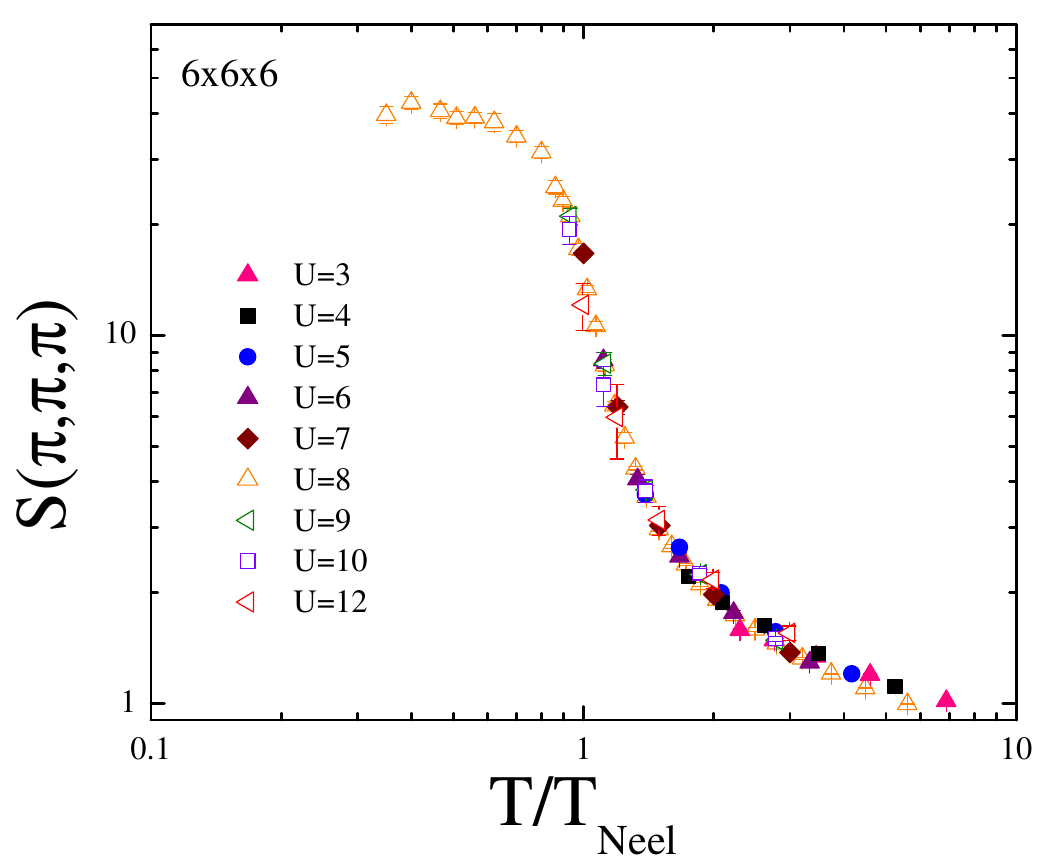
\includegraphics[width=0.6\textwidth]{figures/spilog.png}
\caption{$S_{\pi}$ vs $T/T_{N}$. }
\label{fig:spilog}
\end{figure}
We will see later on that the current LDA results ( which are still not cold
enough to match the experimental data) lead to an effective fraction of 40\%.
So,  for our observed $\bar{S}_{\bv{\pi}}=1.9$  then $ [S_{\pi}]_{\mathrm{max}}
= 3.3  $, which would imply that the lowest local $T/T_{N}$  in our cloud is
$T/T_{N} \approx 1.5$ according to QMC calculations by Thereza,  cf.
Fig.~\ref{fig:spilog}.  

So at the moment the best claim we can make is $T/T_{N}
< 1.5$. 
 

\section{ NLCE data }

Ehsan has provided us with exact NLCE (numerical linked-cluster expansion) data
down to $T/t=1.6$.  Below this temperature he can do a resummation to obtain
the thermodynamic quantities.  At values of the temperature around $T/t=0.4$ the
results start getting very noisy, however we can recover a usable data set by
applying a low pass filter to the data\footnote{The type of filter used is the
Savitzky-Golay filter
\url{http://www.wire.tu-bs.de/OLDWEB/mameyer/cmr/savgol.pdf}}.  The original
data and the filtered data are shown in Fig.~\ref{fig:NLCE_T0.40}.  Larger
$T/t$ values are less noisy, but the filter is still used up to $T/t=1.4$ to
remove some spurious points that show up in the data.  At $T/t > 1.6$ the data
is exact and it has no spurious points.

%\begin{figure}
%        \centering
%        \begin{subfigure}[t]{0.4\textwidth}
%		\includegraphics[width=\textwidth]{figures/bands1d_V0_firstquant.png}
%\caption{ Band structure when the zero of energy is at the bottom of the
%lattice sites.  The zero of energy does not change with lattice depth, and the
%band energies go up almost like the harmonic oscillator state in an individual
%lattice site.  }
%                \label{fig:Hubbard-firstquant}
%        \end{subfigure}%
%        ~~ %add desired spacing between images, e. g. ~, \quad, \qquad etc.
%          %(or a blank line to force the subfigure onto a new line)
%        \begin{subfigure}[t]{0.4\textwidth}
%		\includegraphics[width=\textwidth]{figures/bands1d_V0_secondquant.png}
%\caption{ Band structure when the zero of energy is at the center of the lowest
%band.  This shift is implicit when the hamiltonian is written in second
%quantized form as in Eq.~\ref{eq:Hubbard-free-secondquant}.  }
%                \label{fig:Hubbard-secondquant}
%        \end{subfigure}
%	\caption{ Band structure in the Hubbard model.  }
%\label{fig:Hubbard-first-second}
%\end{figure}

\begin{figure}
    \centering
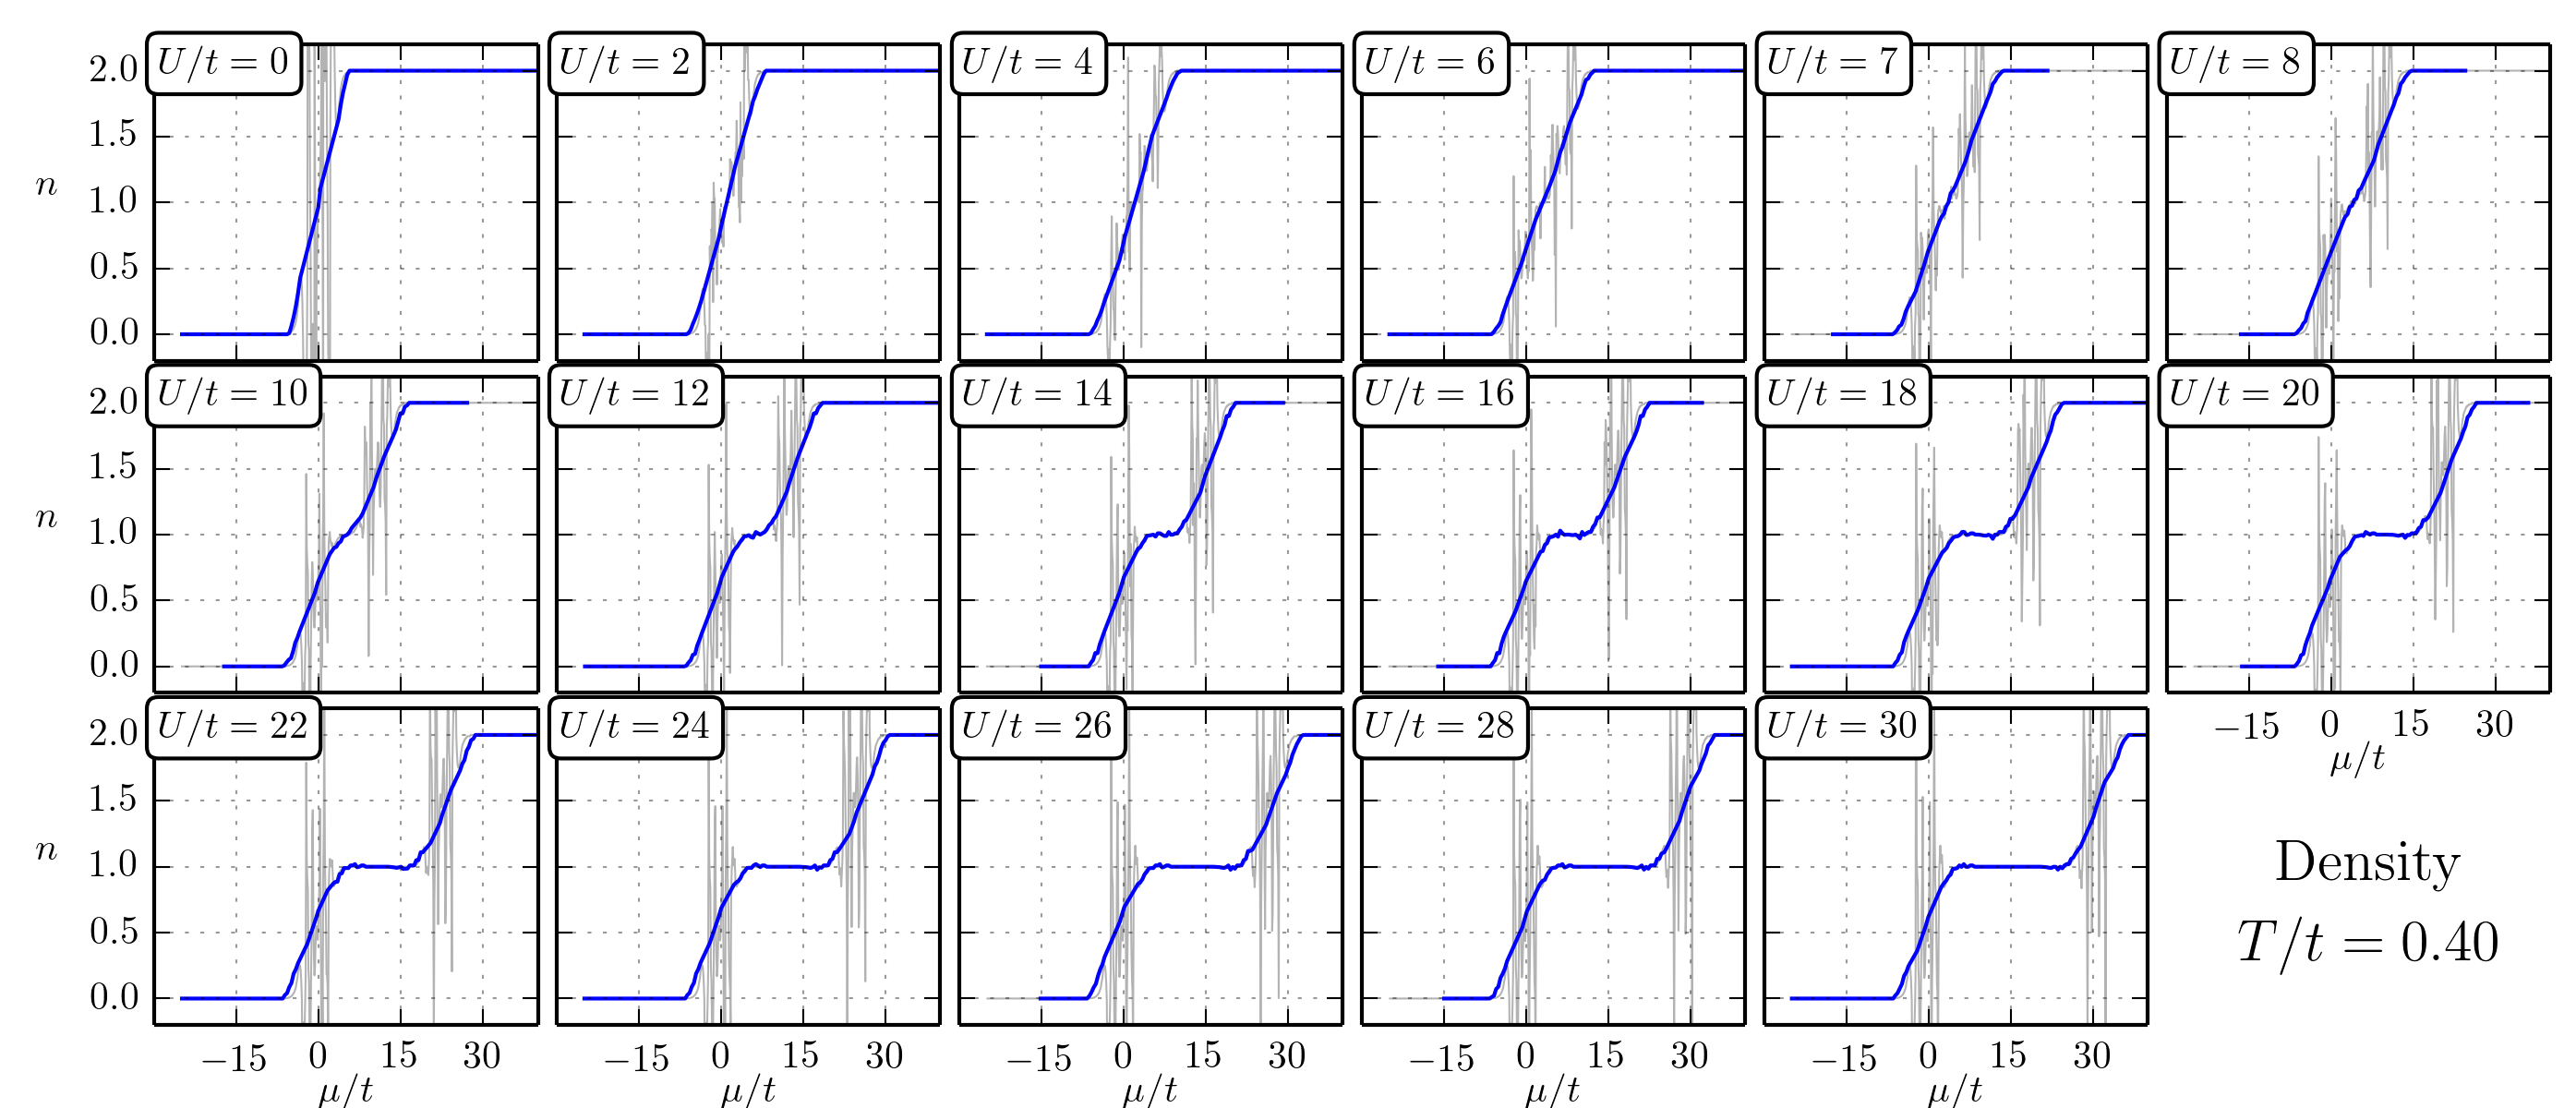
\includegraphics[width=1.0\textwidth]{../dataplots/NLCE_Final/density/T0_40.png}
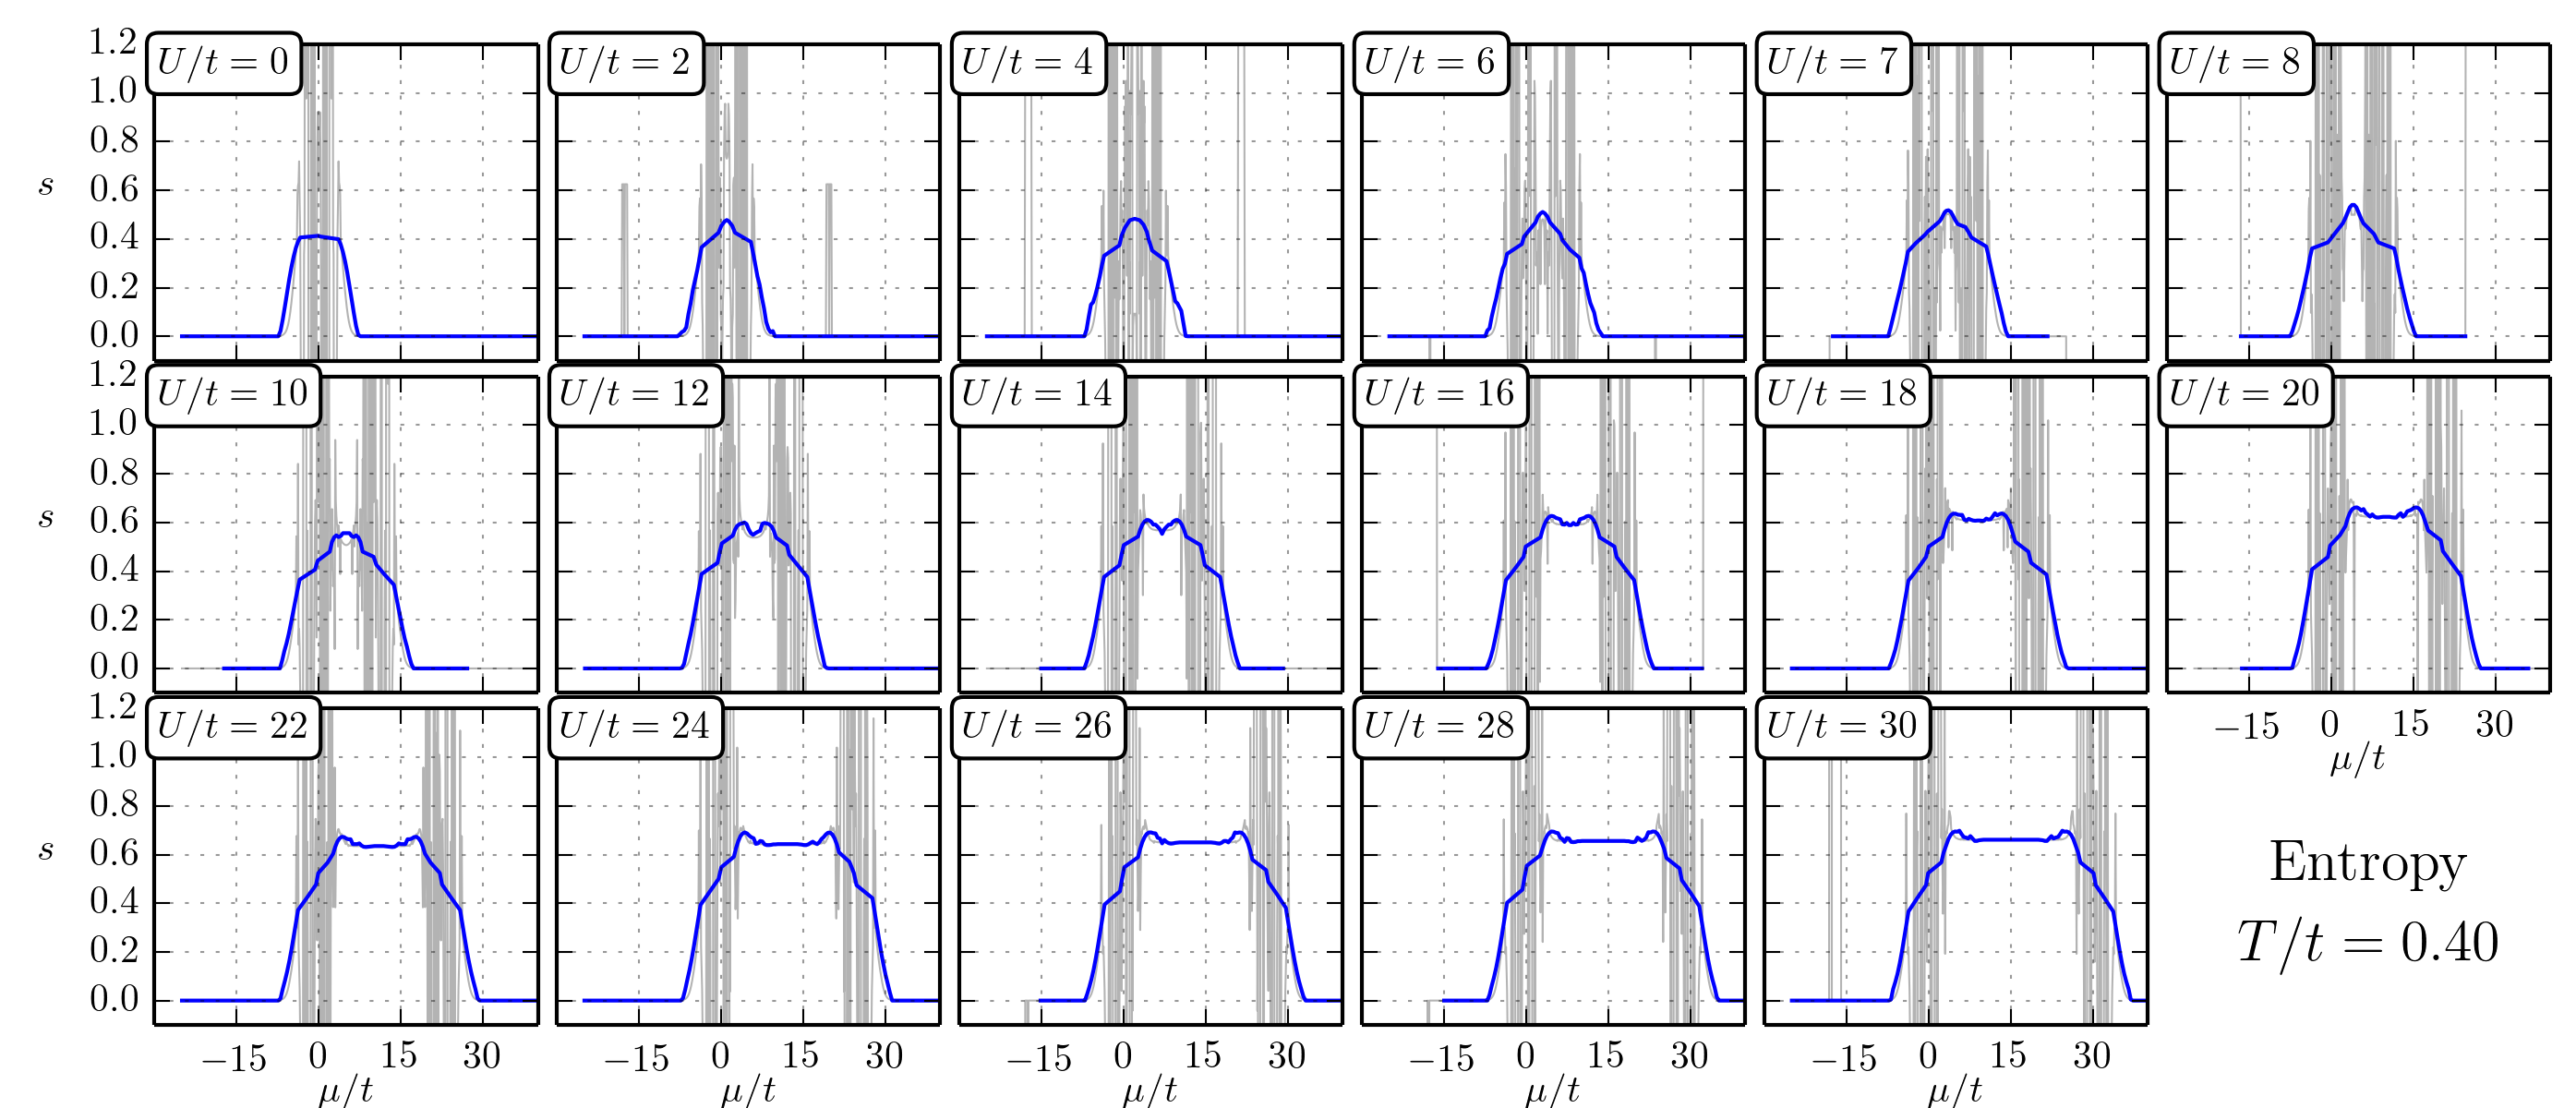
\includegraphics[width=1.0\textwidth]{../dataplots/NLCE_Final/entropy/T0_40.png}
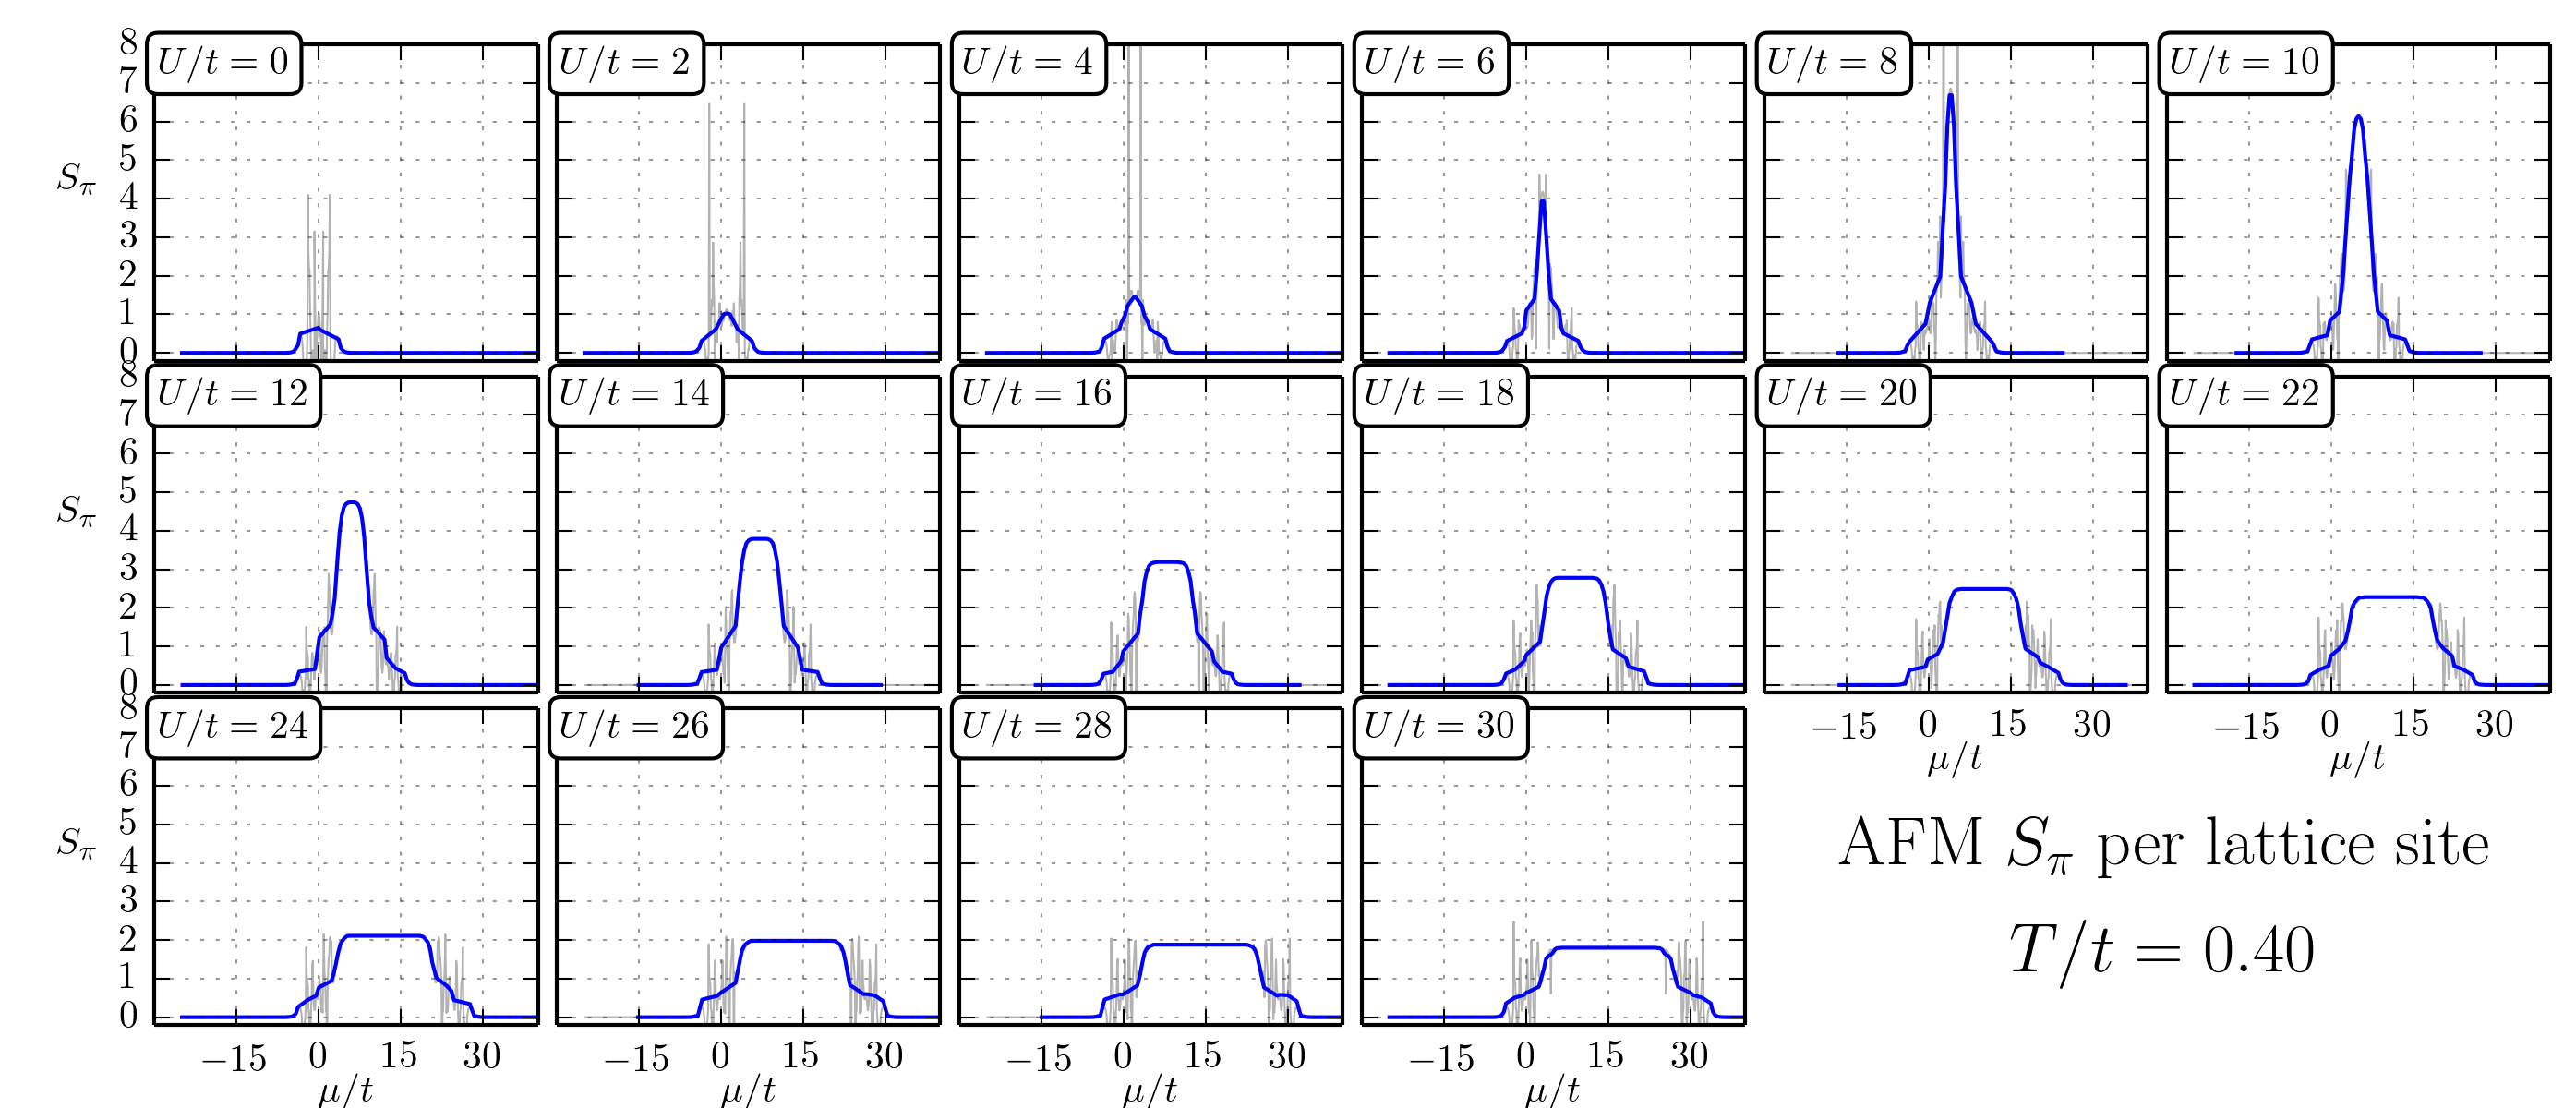
\includegraphics[width=1.0\textwidth]{../dataplots/NLCE_Final/spi/T0_40.png}
\caption{Lowest temperature data accessible to the NLCE by extrapolation,
$T/t=0.4$.  The original data provided by Ehsan is shown in gray and the data
after filtering is shown in blue.}
\label{fig:NLCE_T0.40}
\end{figure}

We can use the NLCE data to see that the density as a function of chemical
potential is pretty much frozen for $T/t<1.0$, see Fig.~\ref{fig:NLCEdens}.
The high temperature series expansion (HTSE) that I was using before to
calculate density profiles works down to about $T/t\approx 1.6$, so I was
unable to capture the ``Mottness'' of the density profile as we see it in the
experiment.
\begin{figure}
    \centering
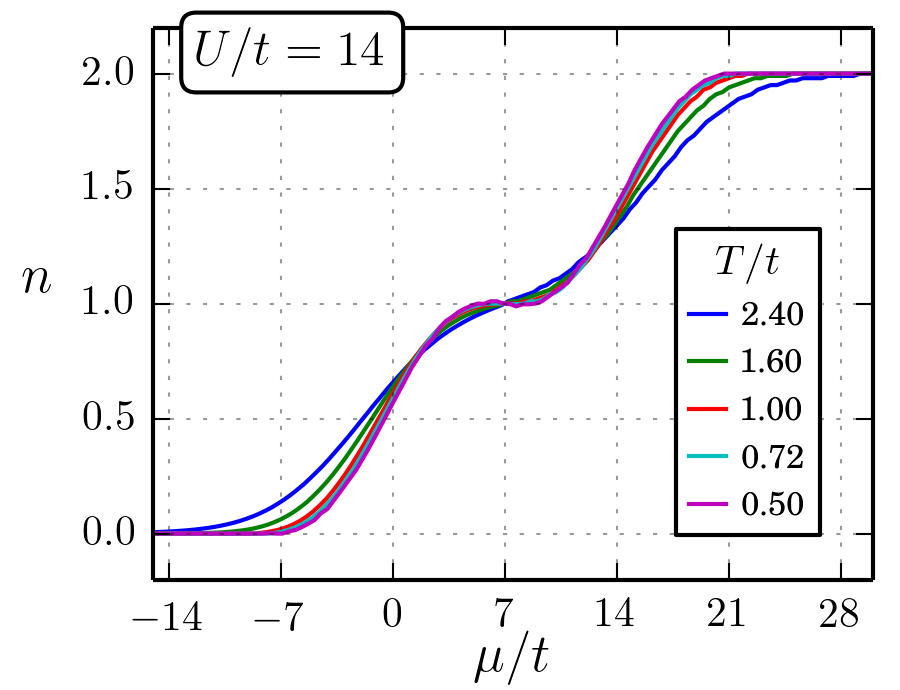
\includegraphics[width=0.6\textwidth]{../dataplots/NLCE_Final/U14_varyT.png}
\caption{NLCE data at $U/t=14$.  For $T/t \leq 1$ the density does not shown
much variation. }
\label{fig:NLCEdens}
\end{figure}


The data for $S_{\bv{\pi}}/n$ provided by NLCE is shown in
Fig.~\ref{fig:NLCESpin}.  Notice that to avoid errors when dividing by a small
value of $n$ we have decided to enforce $S_{\bv{\pi}} = 1$  for densities less
than a density cutoff.  The density cutoff is adjusted for each value of $U/t$.
\begin{figure}
    \centering
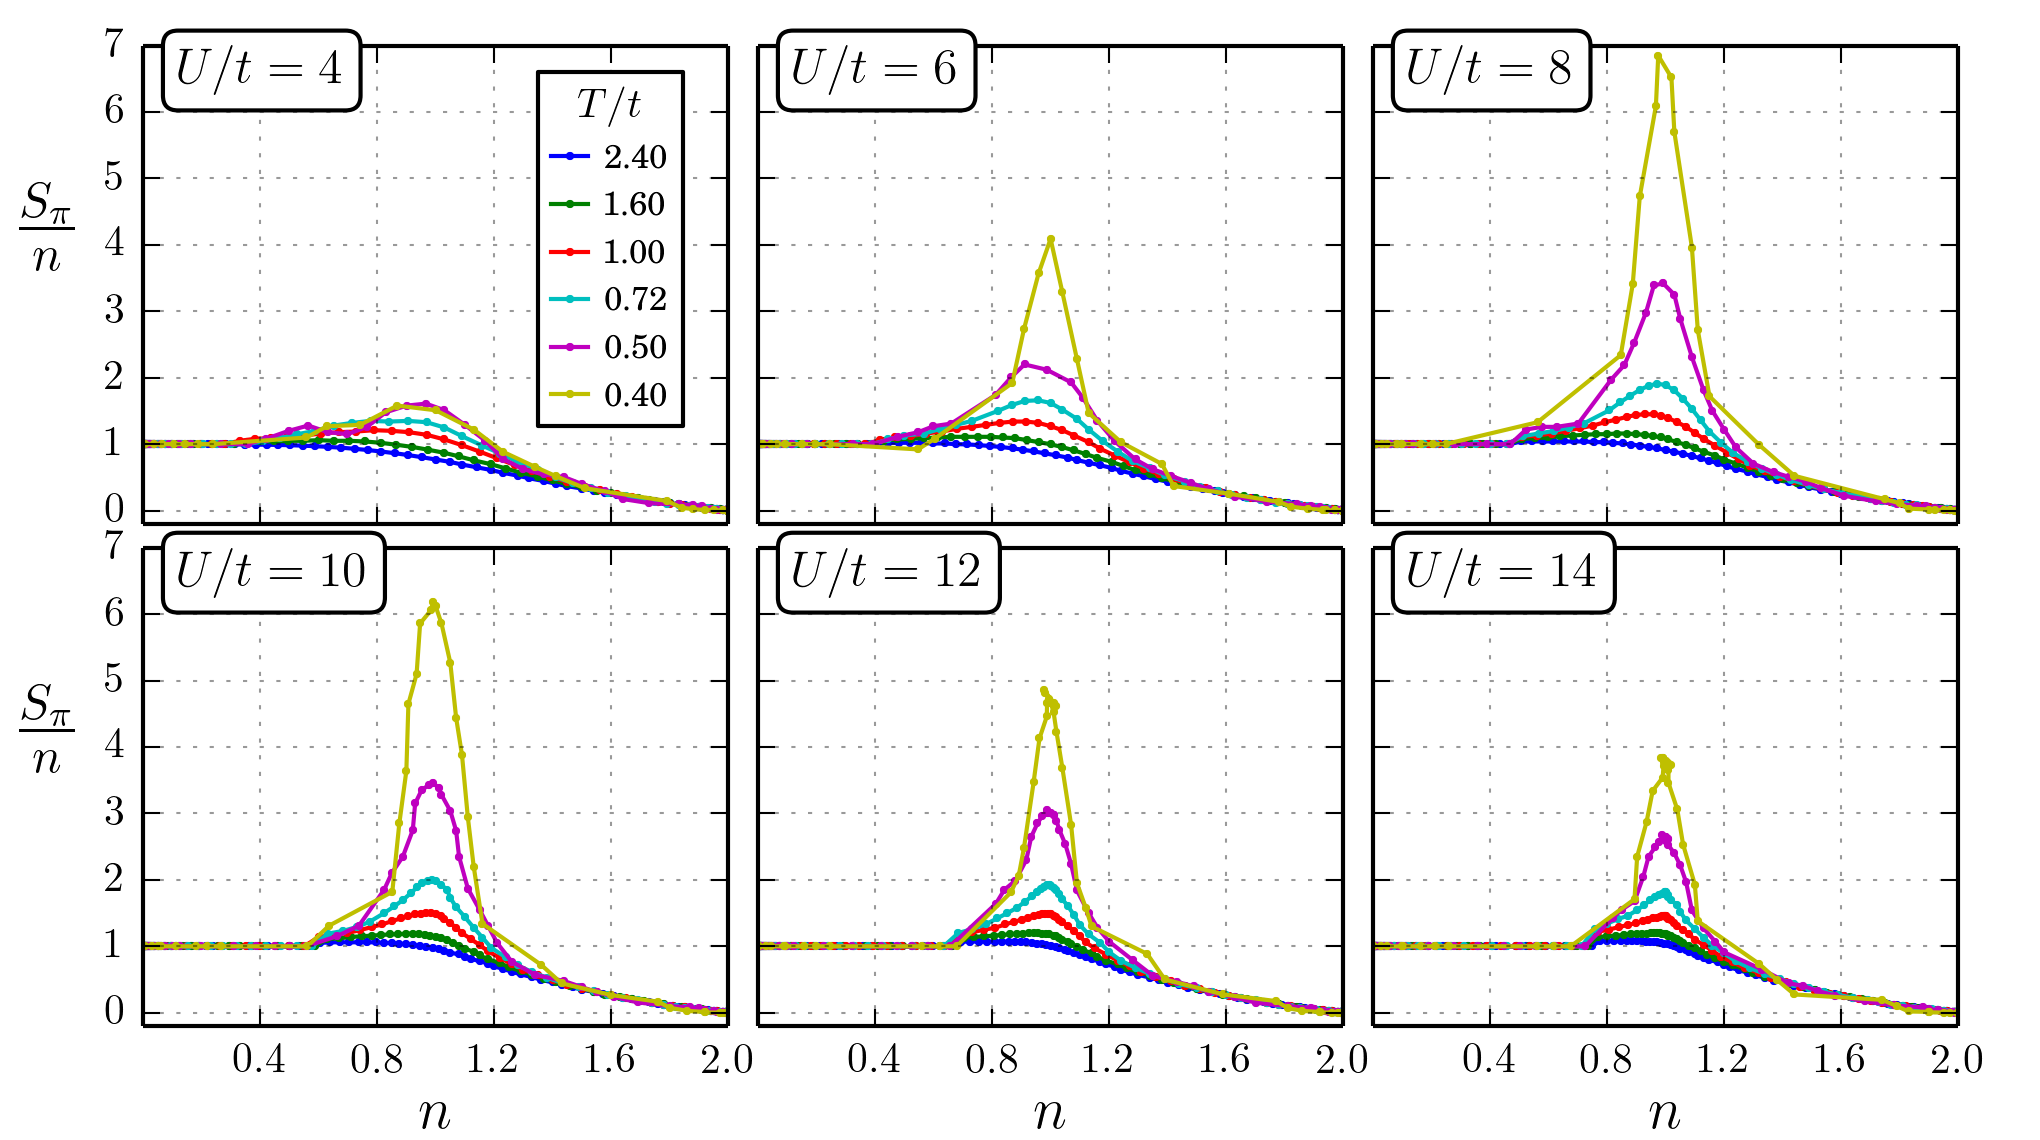
\includegraphics[width=\textwidth]{../dataplots/NLCE_Final/Spi_varyU_varyT.png}
\caption{NLCE $S_{\pi}/n$  data for various interactions and temperatures.  }
\label{fig:NLCESpin}
\end{figure}

\section{ QMC data } 

The QMC data does not suffer from noise problems for small values of $T/t$,
however there is much less of it available.  Fig.~\ref{fig:QMCall} shows the
available $U/t$ and $T/t$ values.  The entropy and double occupancy, not shown
in the Figure are also available from Thereza's data set,  as well as the
structure factor in the $\bv{\theta}$ direction. 
\begin{figure}
    \centering
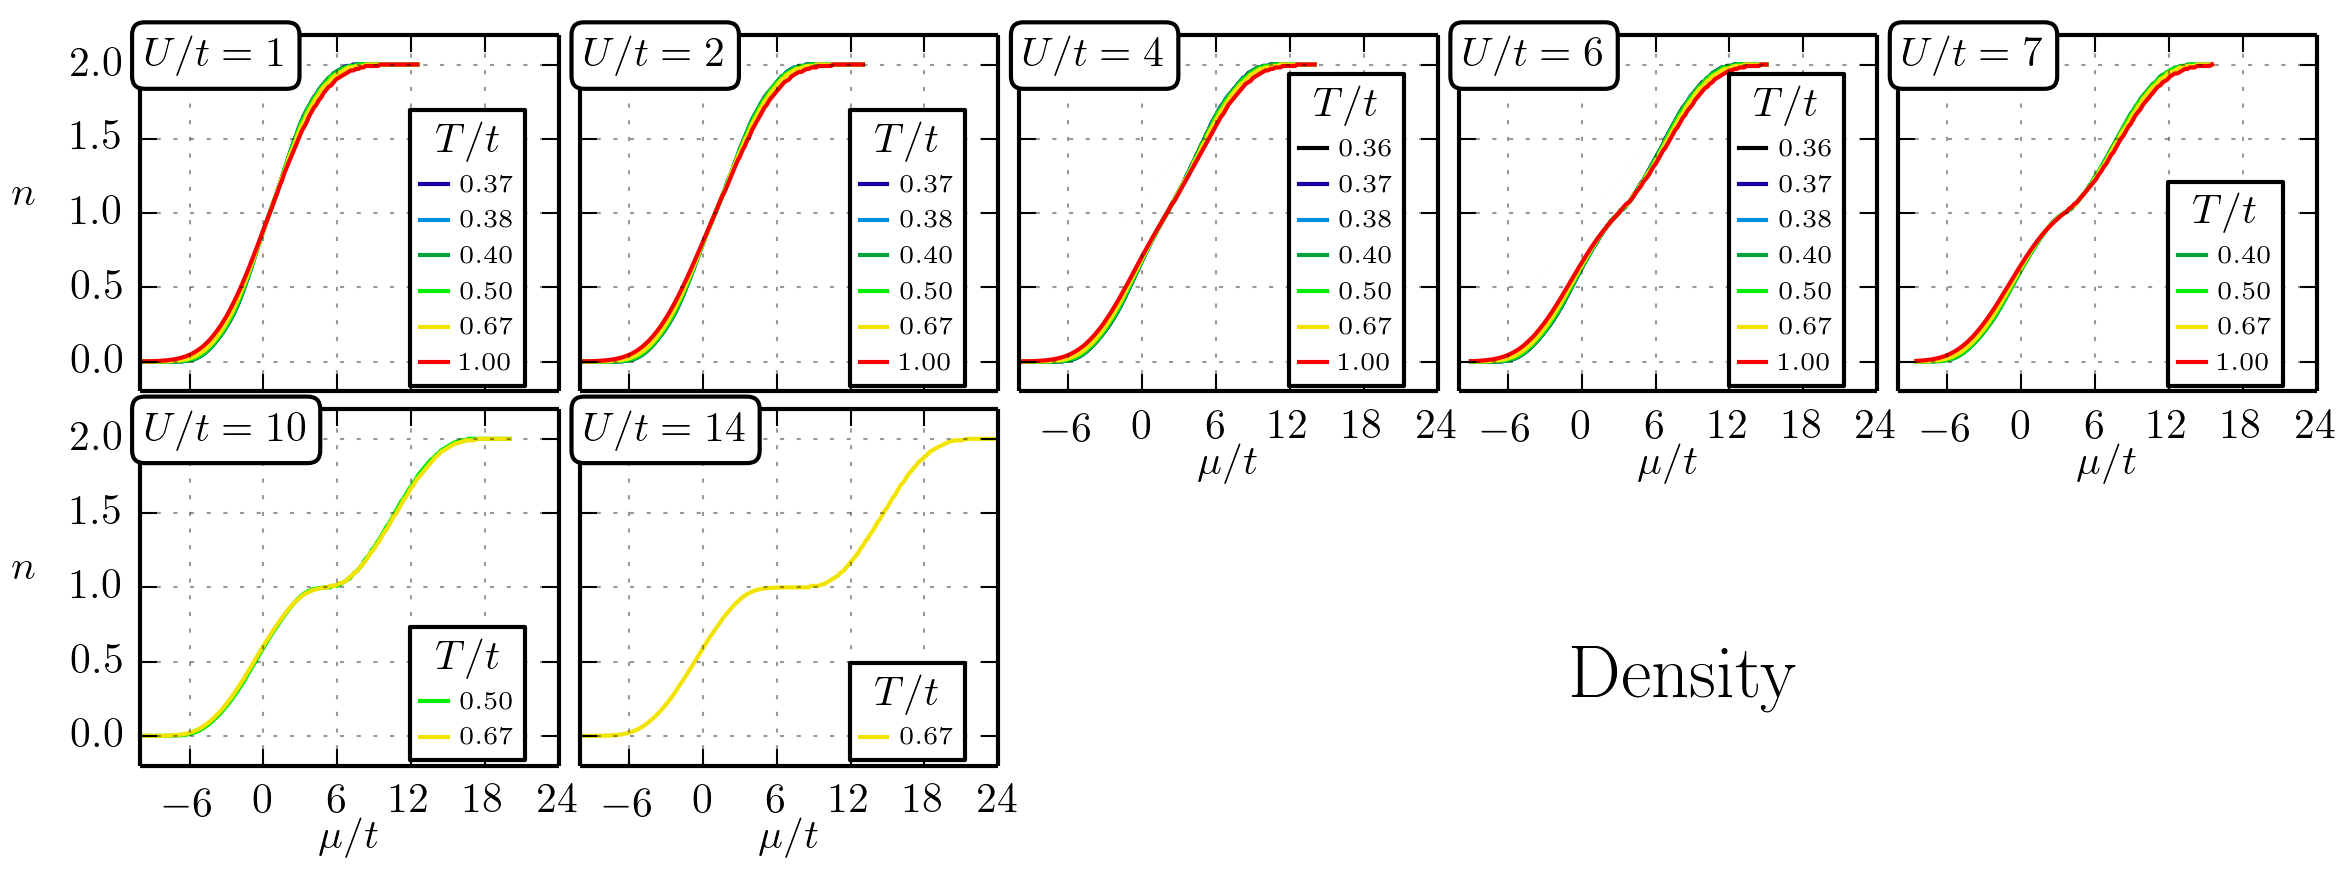
\includegraphics[width=\textwidth]{../dataplots/QMC_Final/density_All.png}
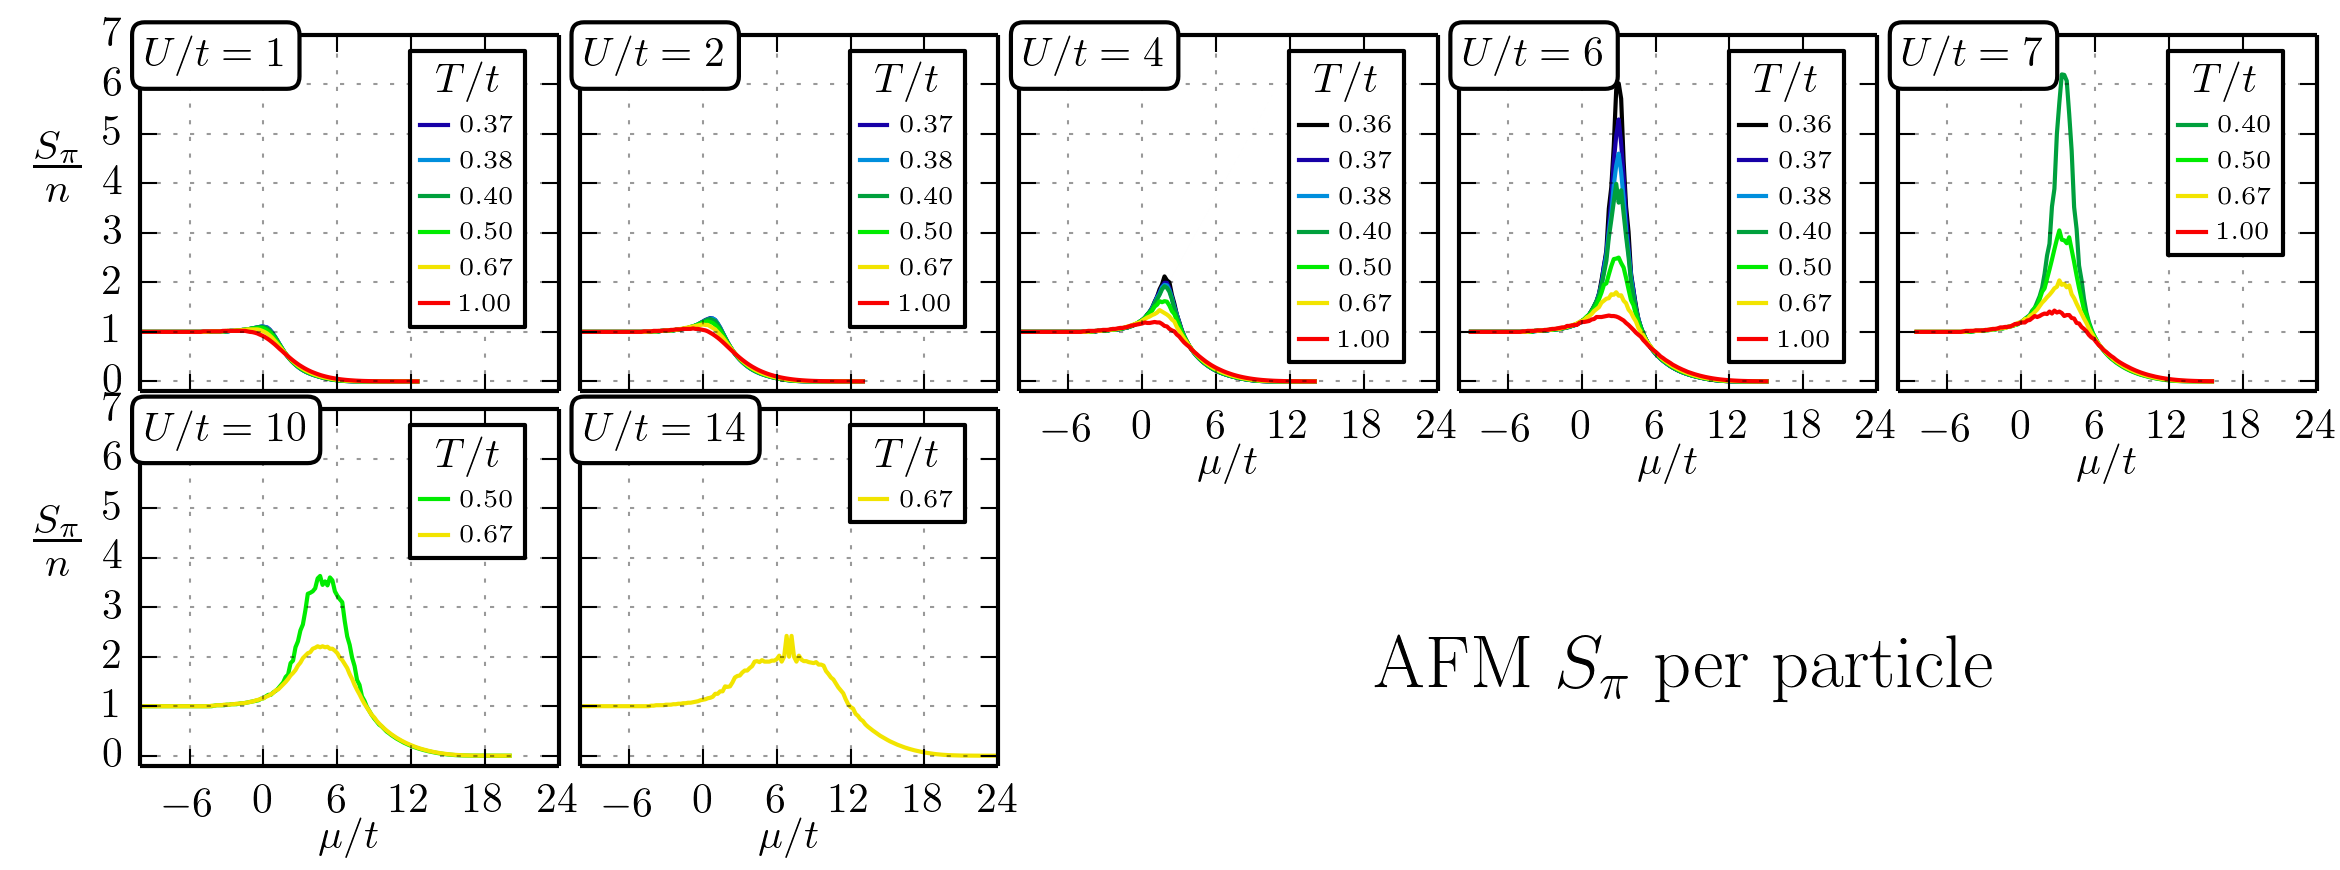
\includegraphics[width=\textwidth]{../dataplots/QMC_Final/spi_n_All.png}
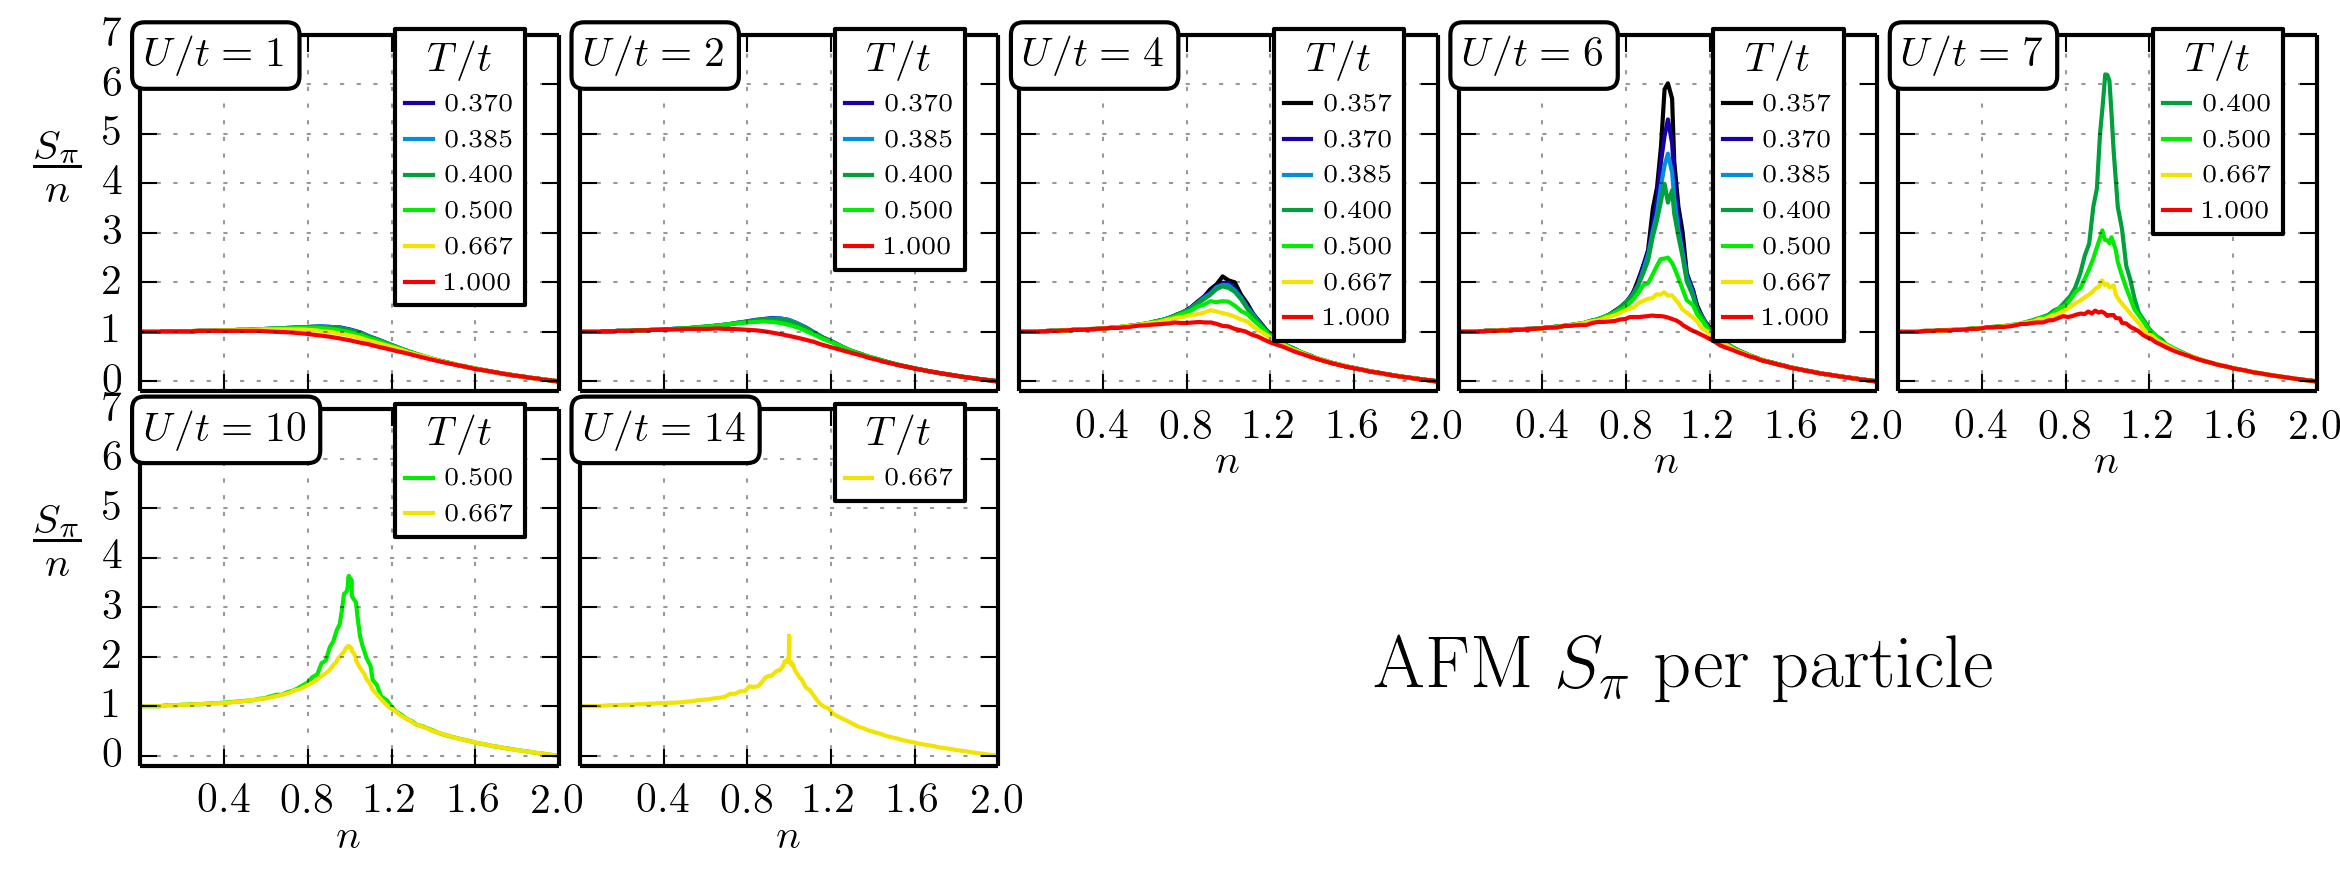
\includegraphics[width=\textwidth]{../dataplots/QMC_Final/spi_n_n_All.png}
\caption{All available QMC data for the density, $S_{\bv{\pi}}$ and
$S_{\bv{\pi}}/n$.  Entropy, double occupancy and  $S_{\theta}/n$ are available
but not shown here.  }
\label{fig:QMCall}
\end{figure}


\section{ NLCE data and QMC data comparison} 

In Fig.~\ref{fig:QMCvsNLCE} we show QMC and NLCE data sets on the same
plot.  A direct comparison is possible at $U/t=6$.  The QMC data at
$U/t=7$ is compared with NLCE at $U/t=8$ which reveals that the NLCE structure
factor is perhaps too broad as a function of $n$.   It is clear from this plots
that the density is frozen for $T/t < 1.0$ and that both QMC and NLCE have very
good agreement on the density. 
\begin{figure}
    \centering
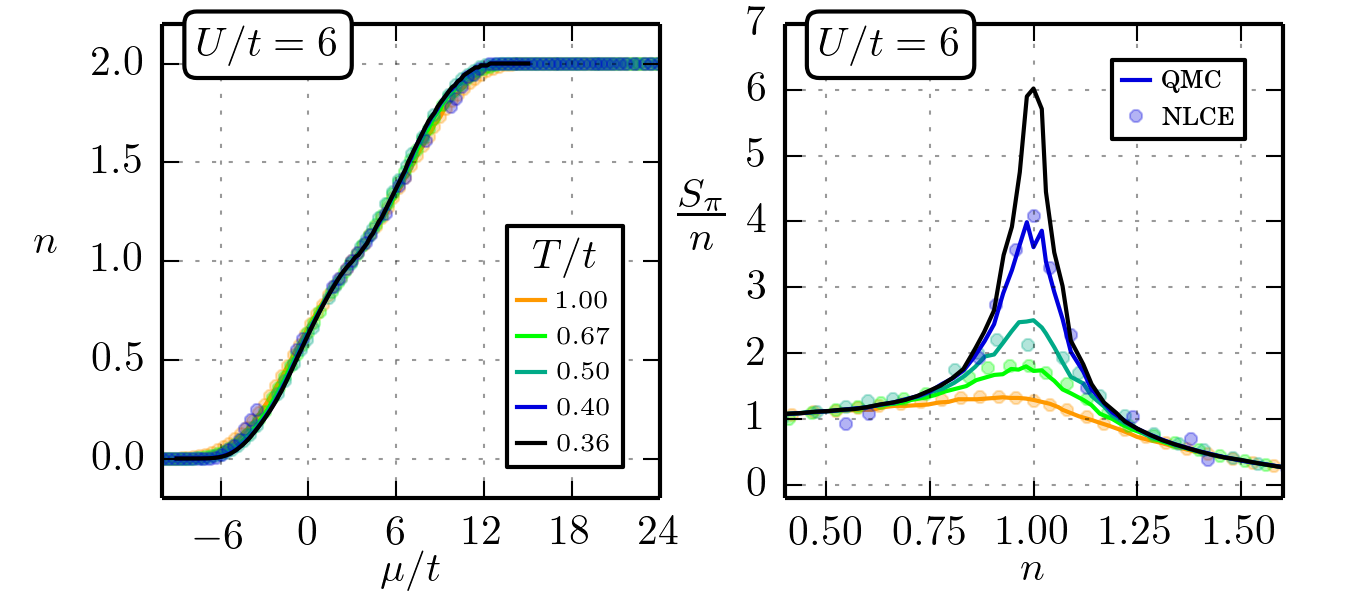
\includegraphics[width=\textwidth]{../dataplots/QMC_Final/QMC_NLCE_Compare_U06.png}
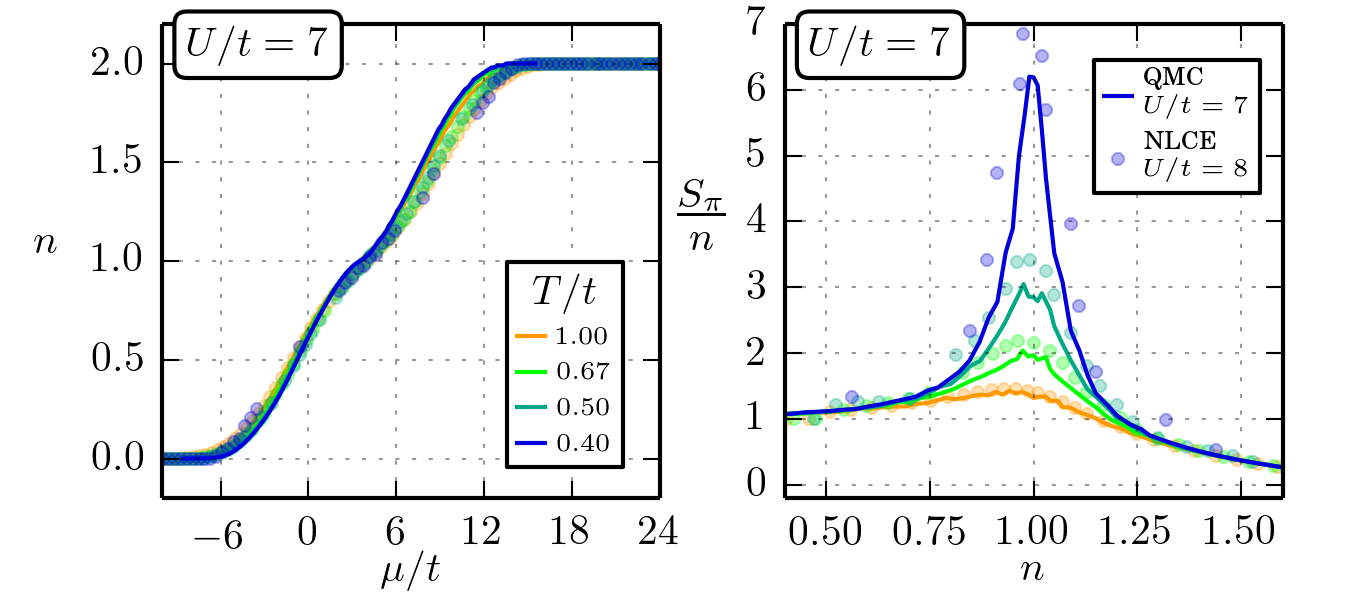
\includegraphics[width=\textwidth]{../dataplots/QMC_Final/QMC_NLCE_Compare_U07.png}
\caption{Comparison between QMC and NLCE data.  At $U/t=6$ both methods have
data available whereas the QMC data at $U/t=7$ is compared with the NLCE data
at $U/t=8$.}
\label{fig:QMCvsNLCE}
\end{figure}


\section{ Comparison of experimental data with LDA } 

The way we will proceed is as follows:

\begin{enumerate}

  \item Set up a trap geometry based on our experimental calibration.  The trap
geometry determines the local chemical potential, the local $U/t$ and the local
$T/t$. 

  \item Use the NLCE data to find the global chemical potential that produces
the desired atom number $N$.   The temperature used simply needs to be $T/t <
1.0$, since $n(\mu)$ is frozen below this temperature.   

  \item For the local $S_{\bv{\pi}}/n$ determination, set a value of
$[T/t]_{0}$.  This is the local value of $T/t$ at the center of the trap.  Use
the global chemical potential (from 2) along with the local $U/t$ and $T/t$ to
get the local $S_{\pi}/n$ via interpolation from available QMC and NLCE data.
 
  \item Integrate the local $S_{\bv{\pi}}/n$ over the trap to obtain the bulk spin
structure factor $\bar{S}_{\bv{\pi}}$. 

  \item Repeat 3 and 4 for decreasing values of $[T/t]_{0}$ until the resulting
$\bar{S}_{\bv{\pi}}$ agrees with the experimental measurement.  
\end{enumerate}

\subsection{ Determination of $S_{\bv{\pi}}/n$  by interpolation} 

We use a combination of the available QMC and NLCE data set to find out
$S_{\bv{\pi}}/n$ for given local values of  $\mu/t$, $U/t$, and $T/t$.   To allow
evaluation for arbitrary values of the parameters we interpolate linearly
between the available data points.  An example is shown in
Fig.~\ref{fig:interp}.  

\begin{figure}
    \centering
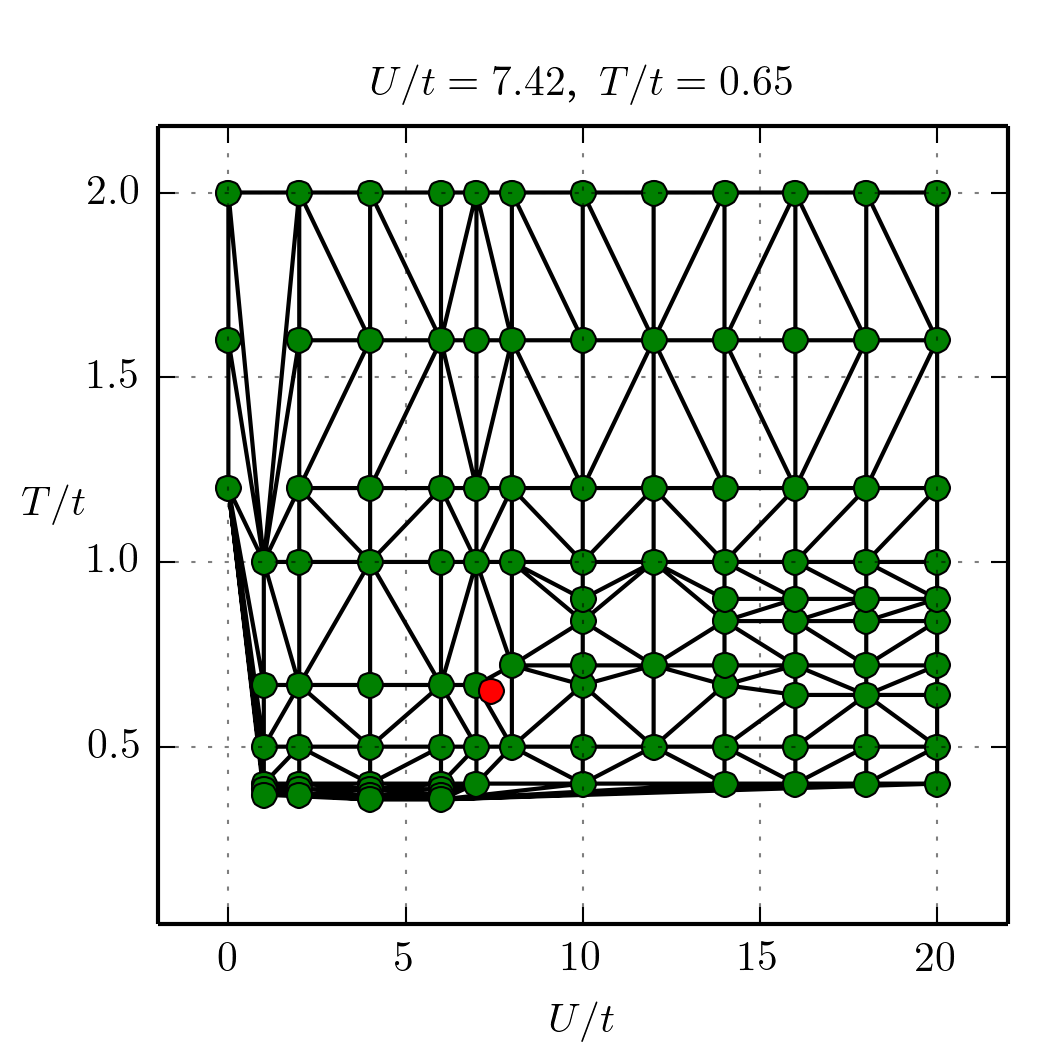
\includegraphics[width=0.48\textwidth]{../dataplots/interp/allpts.png}
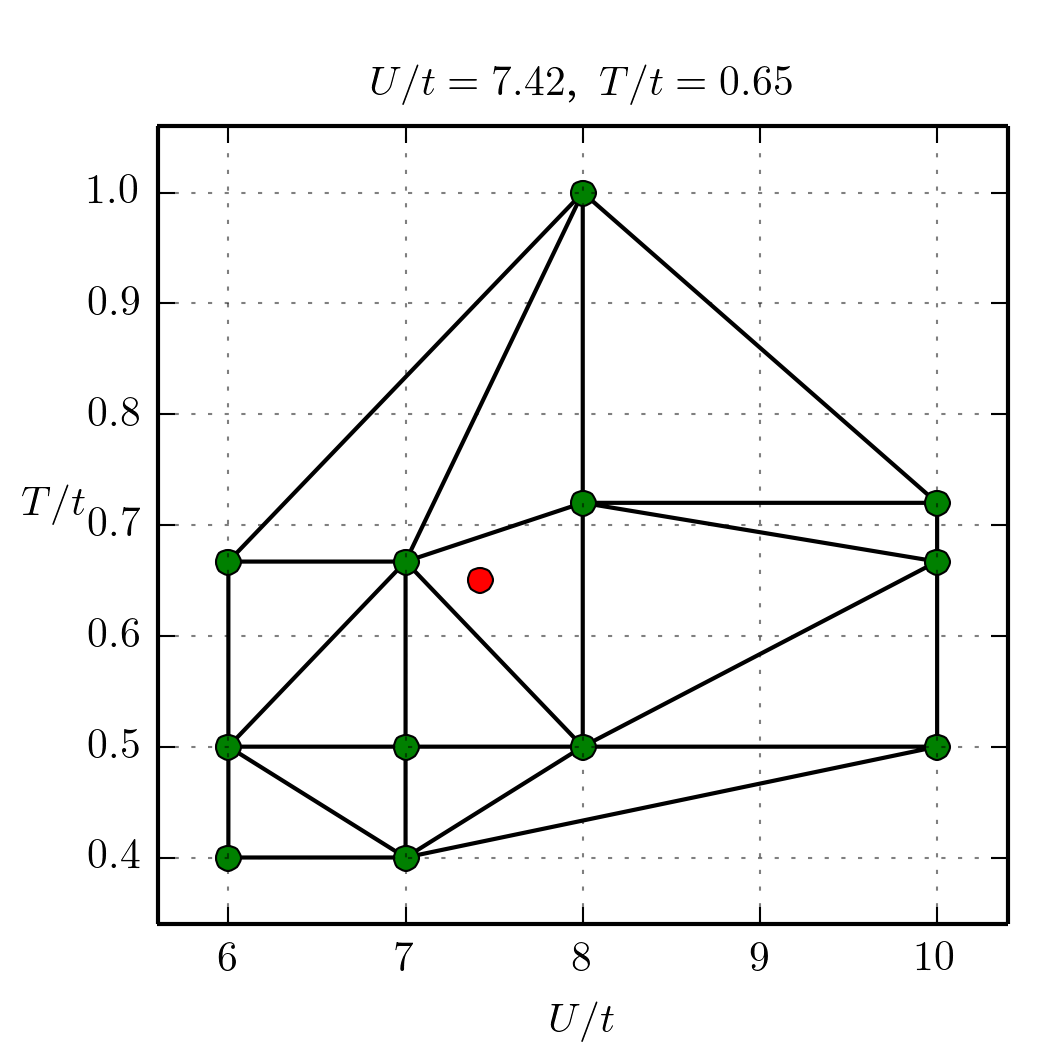
\includegraphics[width=0.48\textwidth]{../dataplots/interp/closepts.png}
\caption{ Illustration of linear interpolation.  Left panel shows all available
points from a combination of QMC and NCE data sets. Right panel shows a close
up view and the triangulation scheme which is used to linearly interpolate.
The value at the red point is determined by the 3 green points which form the
triangle that enclose it.  Note that the value of $S_{\bv{\pi}}/n$ at each
green point is obtained from the data tables at the local chemical potential of
interest.   } 
\label{fig:interp}
\end{figure}

\subsection{ LDA density profiles with NLCE data, dependence on $T$}


To illustrate the effect of temperature on the density profile we show in
Fig.~\ref{fig:dens_varyT}  density profiles with $n=1$ at the center,
calculated for various values of $[T/t]_{0}$,  where $[T/t]_{0}$ is the local
value of $T/t$ at the center of the cloud.  The sample is assumed to be
isothermal so it has constant $T$ throughout, the local value of $t$ varies due
to the size of the lattice beams.
\begin{figure}
    \centering
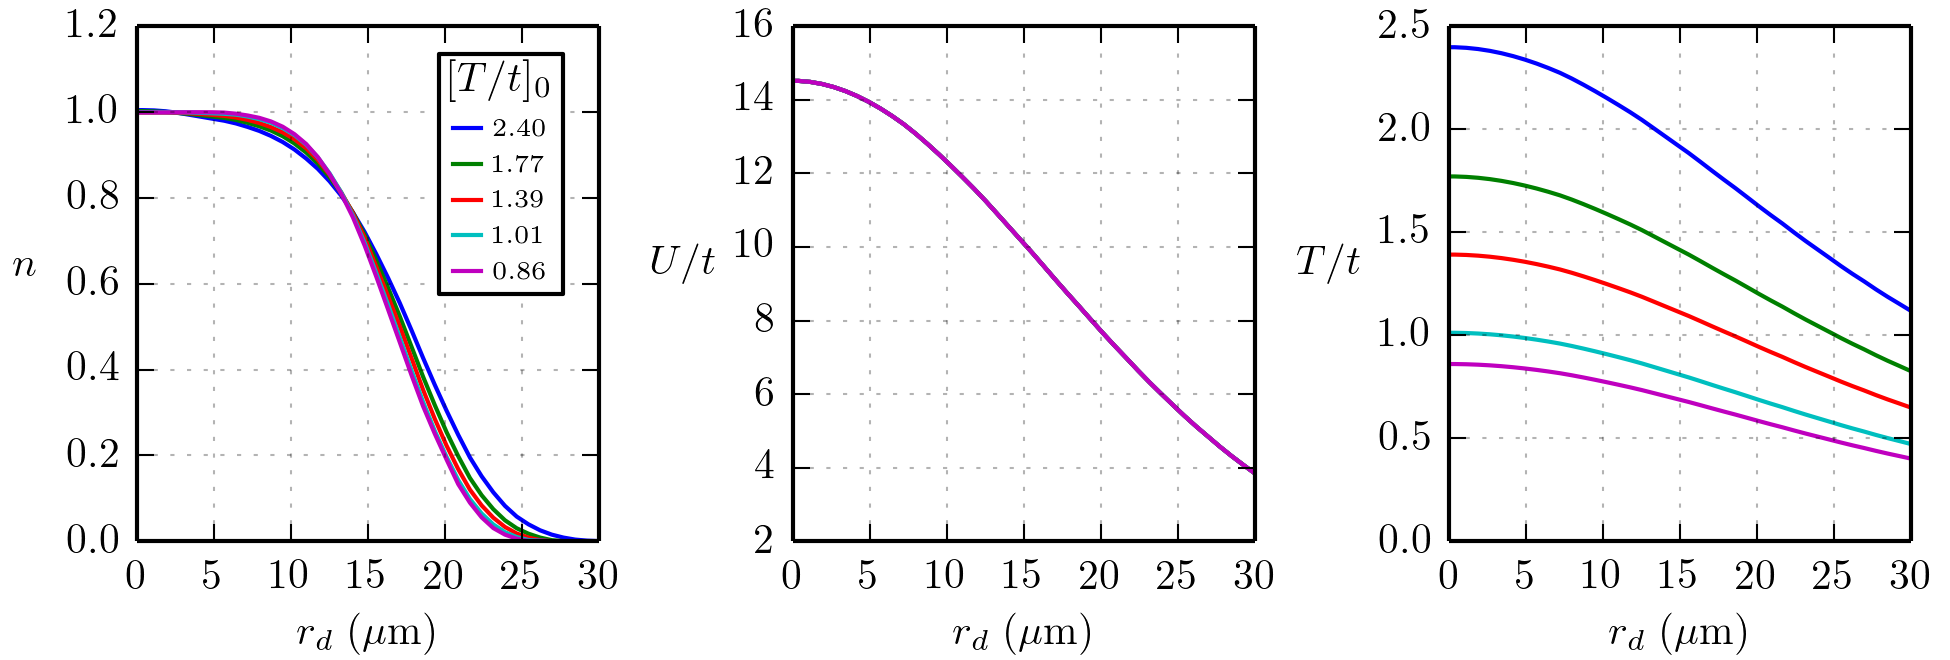
\includegraphics[width=\textwidth]{../dataplots/Basic00/density_varyT.png}
\caption{Density profiles with $n=1$ at the center for various values of
$[T/t]_{0}$. For $[T/t]_{0}<1$ the density profile changes very little with
temperature.  The right two panes show the spatial variation of $U/t$ and $T/t$
across the sample, illustrating the degree of inhomogeneity in the system. }
\label{fig:dens_varyT}
\end{figure}
As expected we see that for $[T/t]_{0} < 1 $ the density profile does not change
very much, which validates our approach of calculating the density profile and
determining the global chemical potential at a single $T/t<1.0$  using
the NLCE data (see step 2 in the prescription outlined above).  


\subsection{ LDA $S_{\pi}/n$ profiles, lowest accessible $T$ variation of $N$} 
 
In the experiment we varied the atom number to maximize the Bragg signal for a
given value of $[U/t]_{0}$.   Here we calculate $S_{\pi}$ profiles for various
atom numbers and show how does the bulk spin structure factor $\bar{S}_{\pi}$
varies with atom number. 


\begin{figure}
    \centering
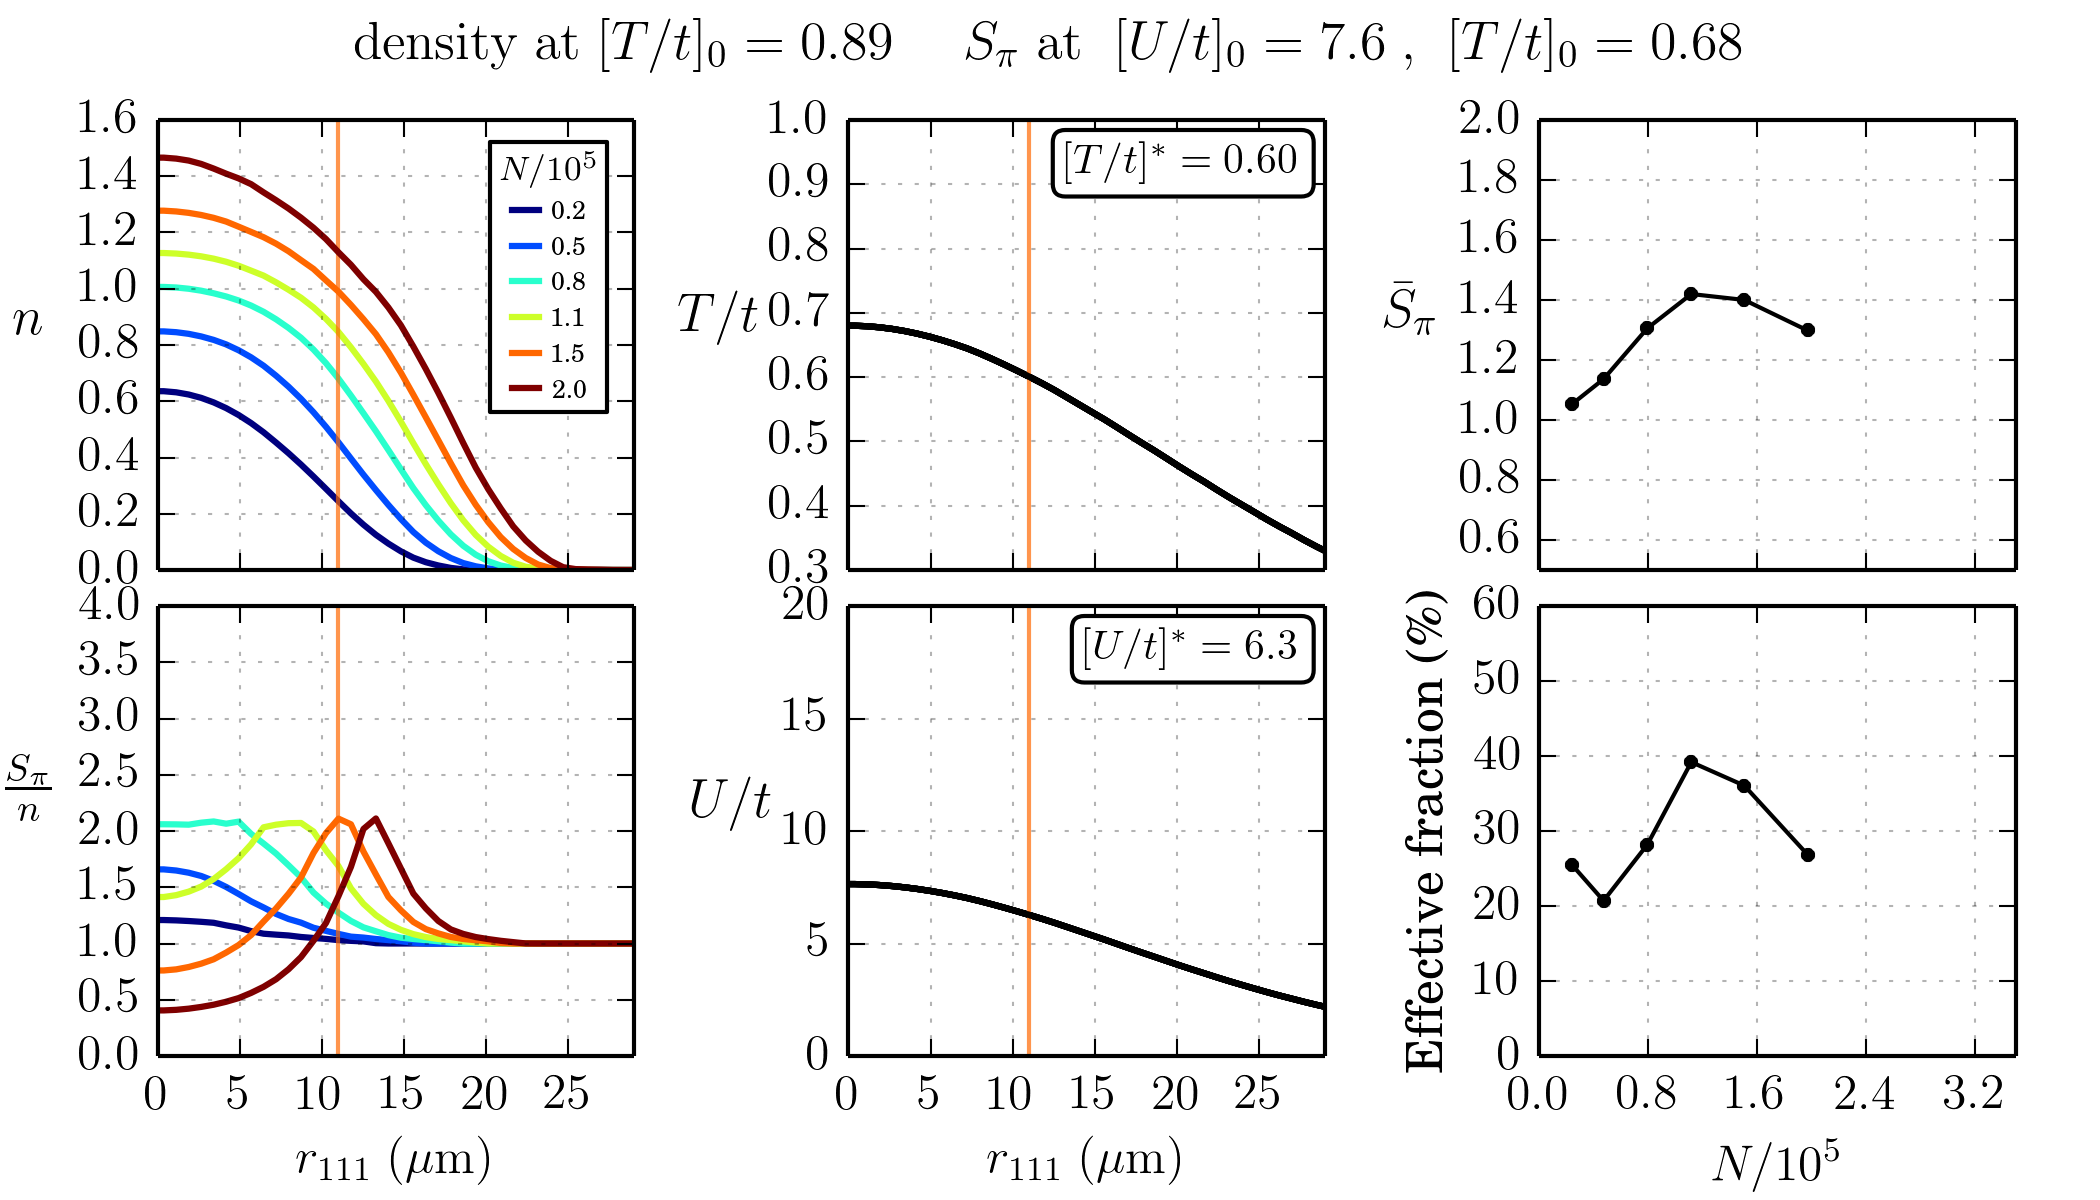
\includegraphics[width=\textwidth]{figures/200a0_cold.png}
\caption{Scattering length 200\,$a_{0}$ ($[U/t]_{0}=7.6$).  Variation of
density profile, $S_{\pi}/n$ profile,  $\bar{S}_{\bv{\pi}}$  and effective
fraction with atom number. } 
\label{fig:200a0_varyN}
\end{figure}

\begin{figure}
    \centering
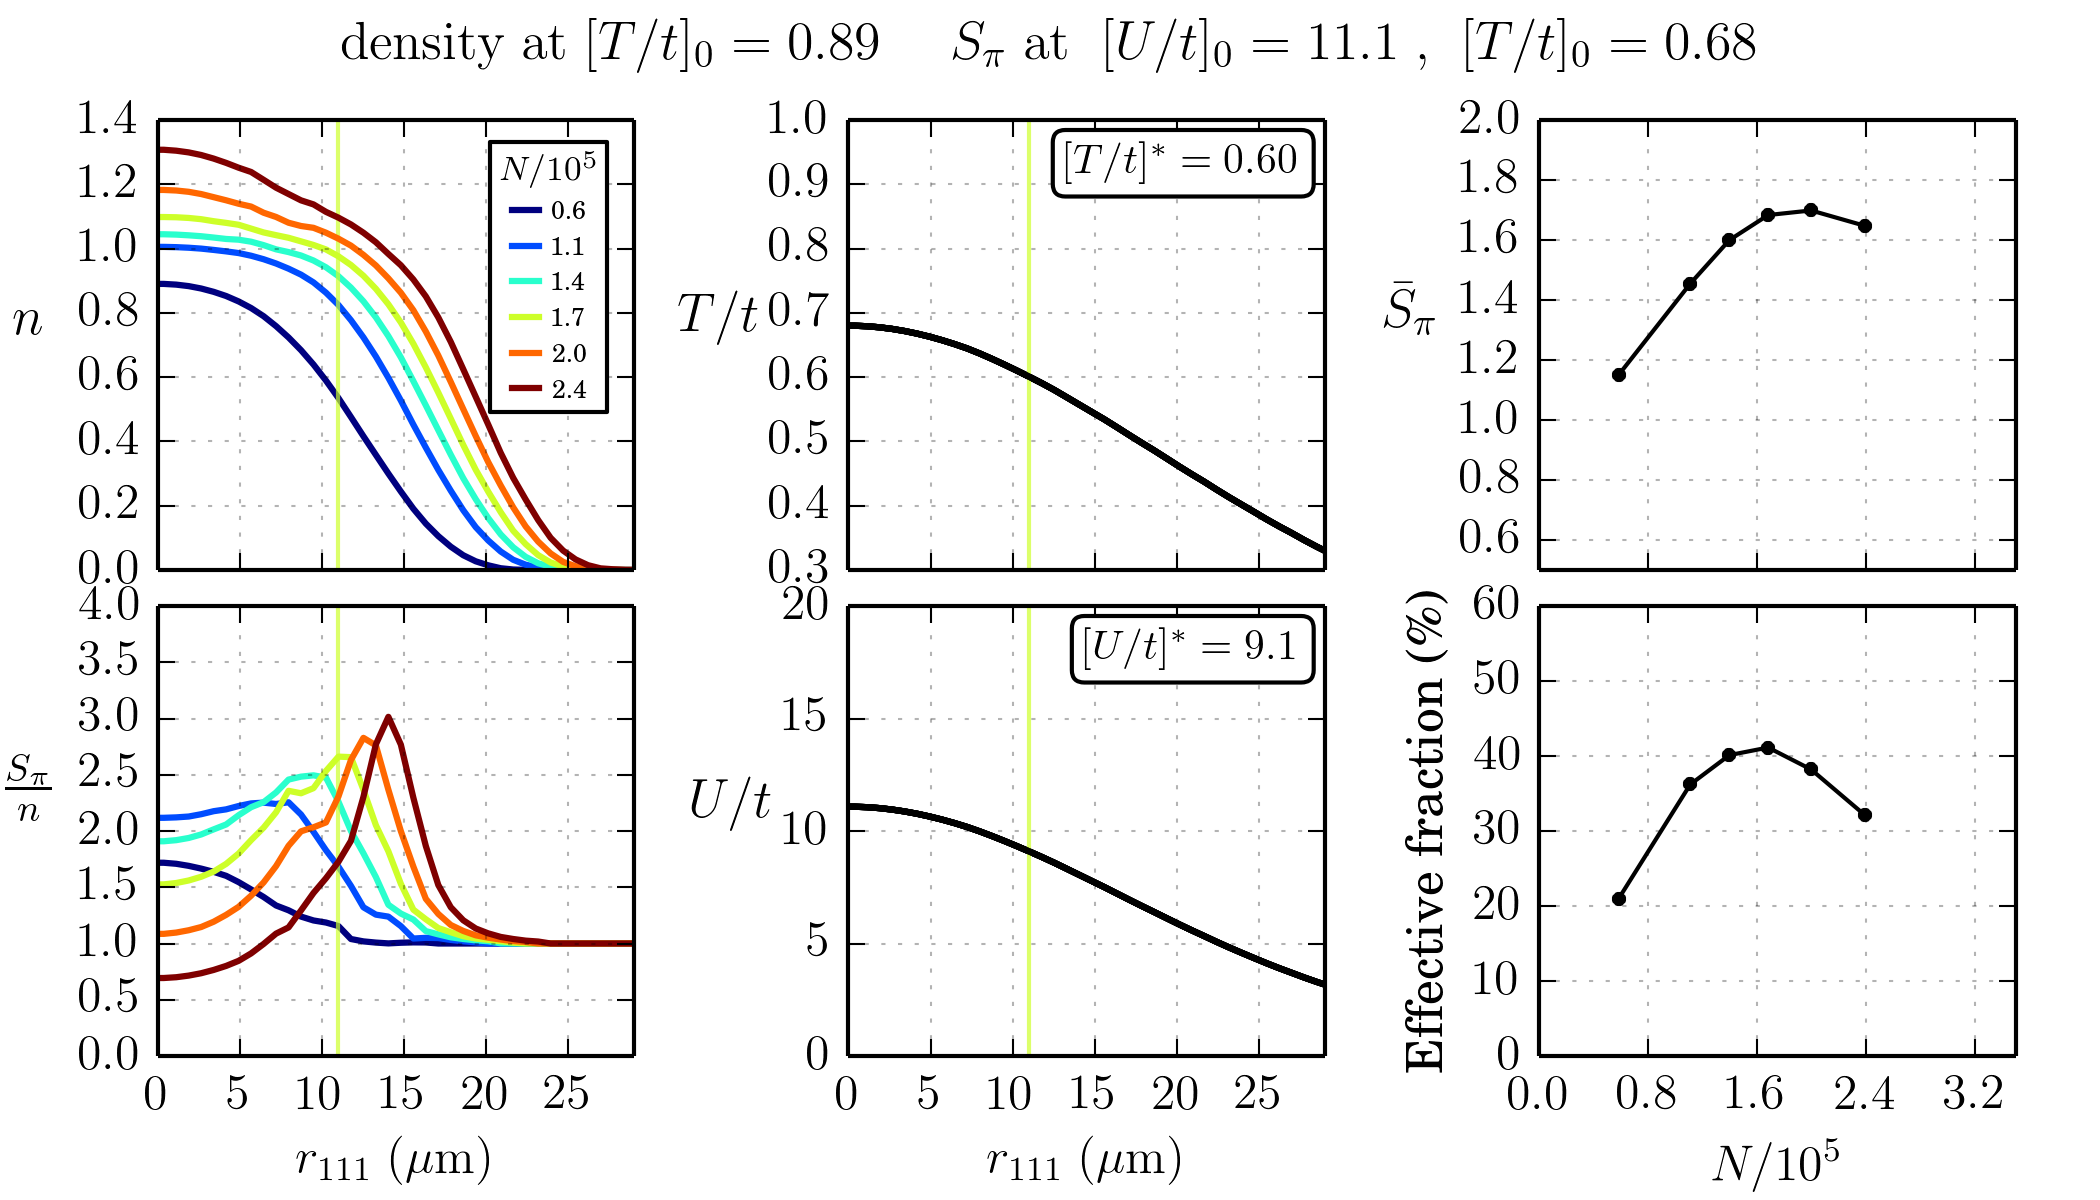
\includegraphics[width=\textwidth]{figures/290a0_cold.png}
\caption{Scattering length 290\,$a_{0}$ ($[U/t]_{0}=11.1$).   } 
\label{fig:290a0_varyN}
\end{figure}

\begin{figure}
    \centering
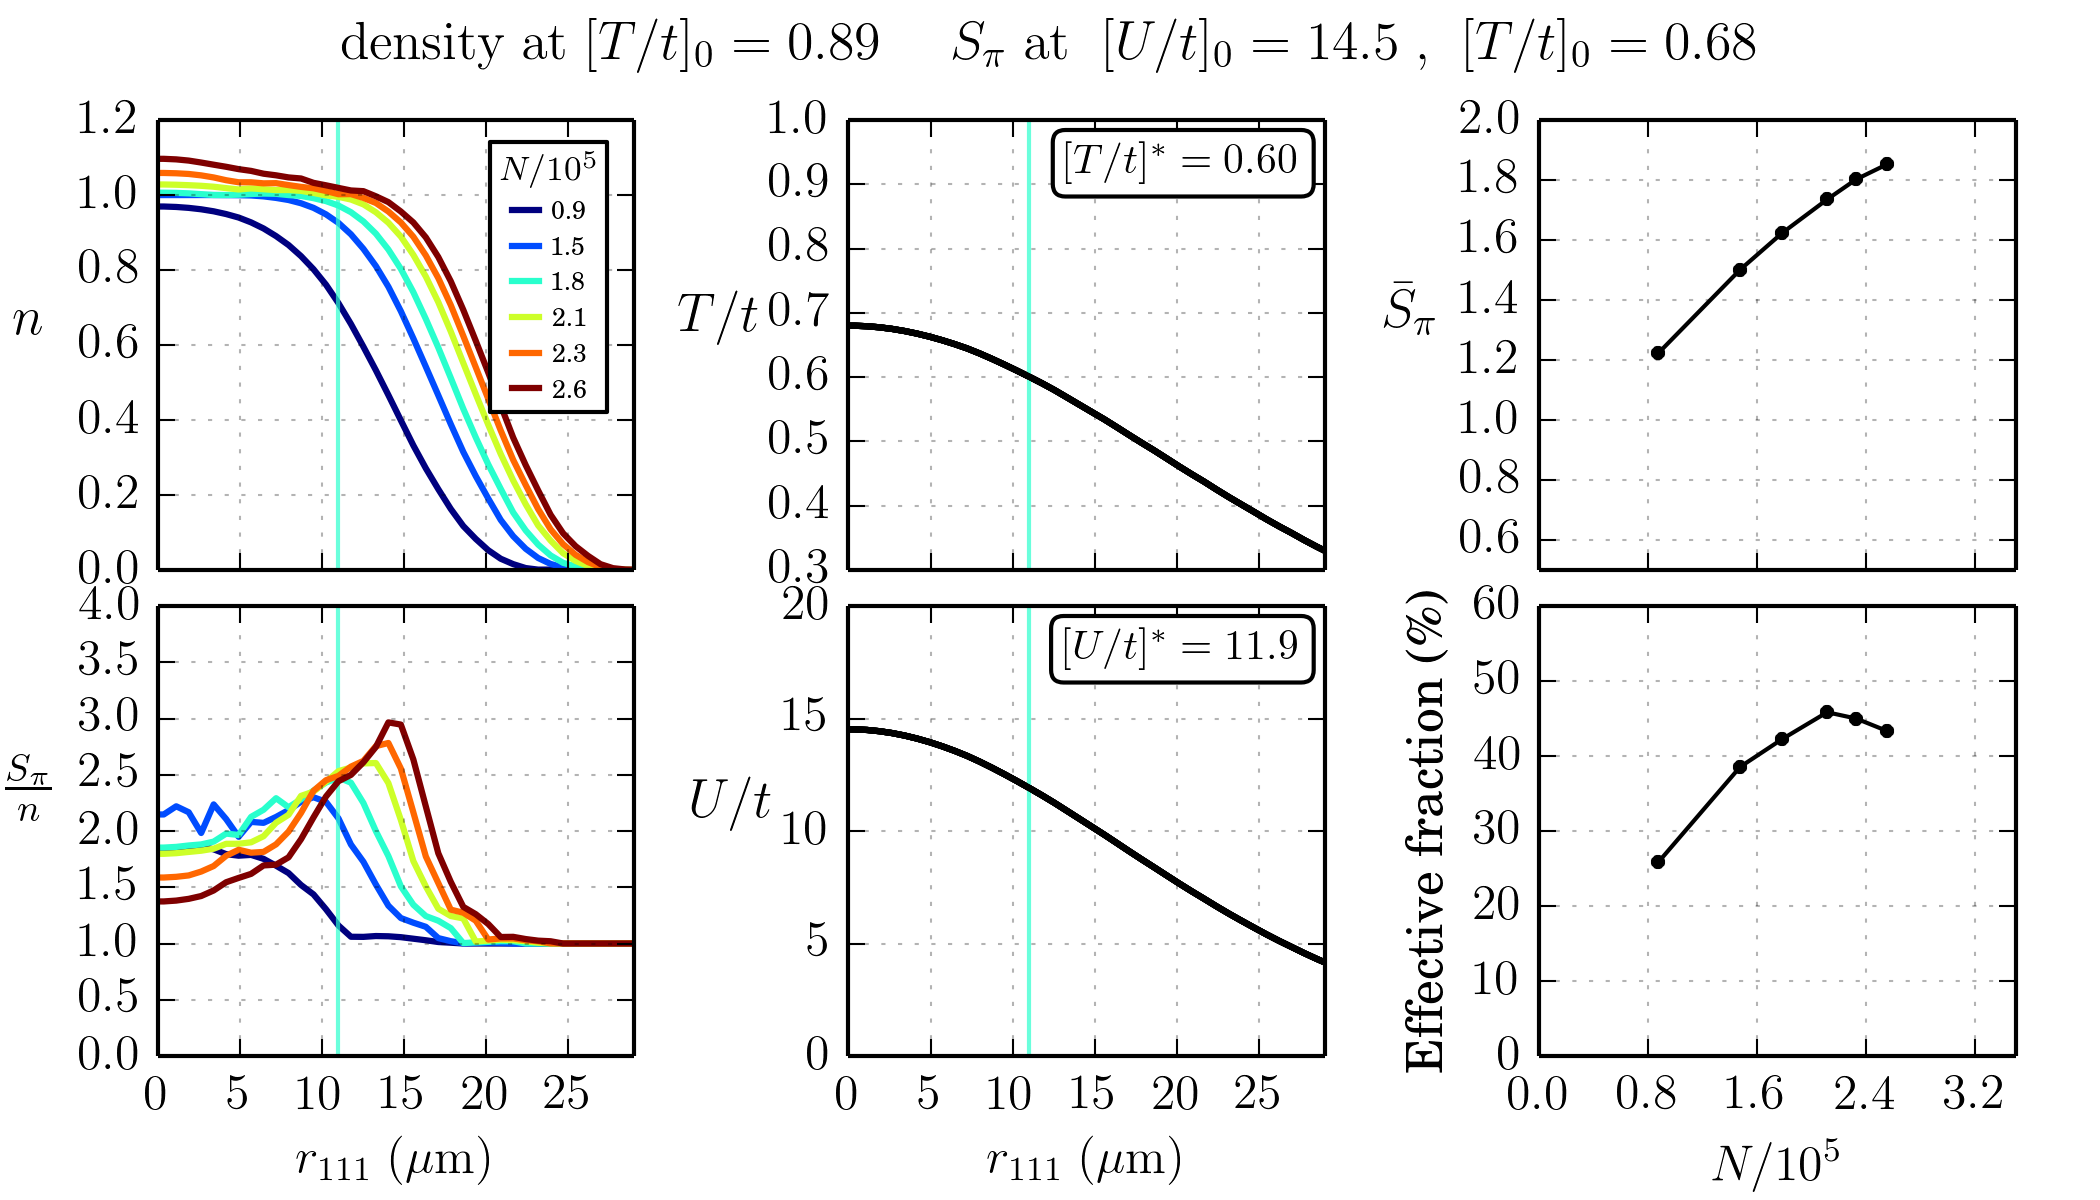
\includegraphics[width=\textwidth]{figures/380a0_cold.png}
\caption{Scattering length 380\,$a_{0}$ ($[U/t]_{0}=14.5$).   } 
\label{fig:380a0_varyN}
\end{figure}

\begin{figure}
    \centering
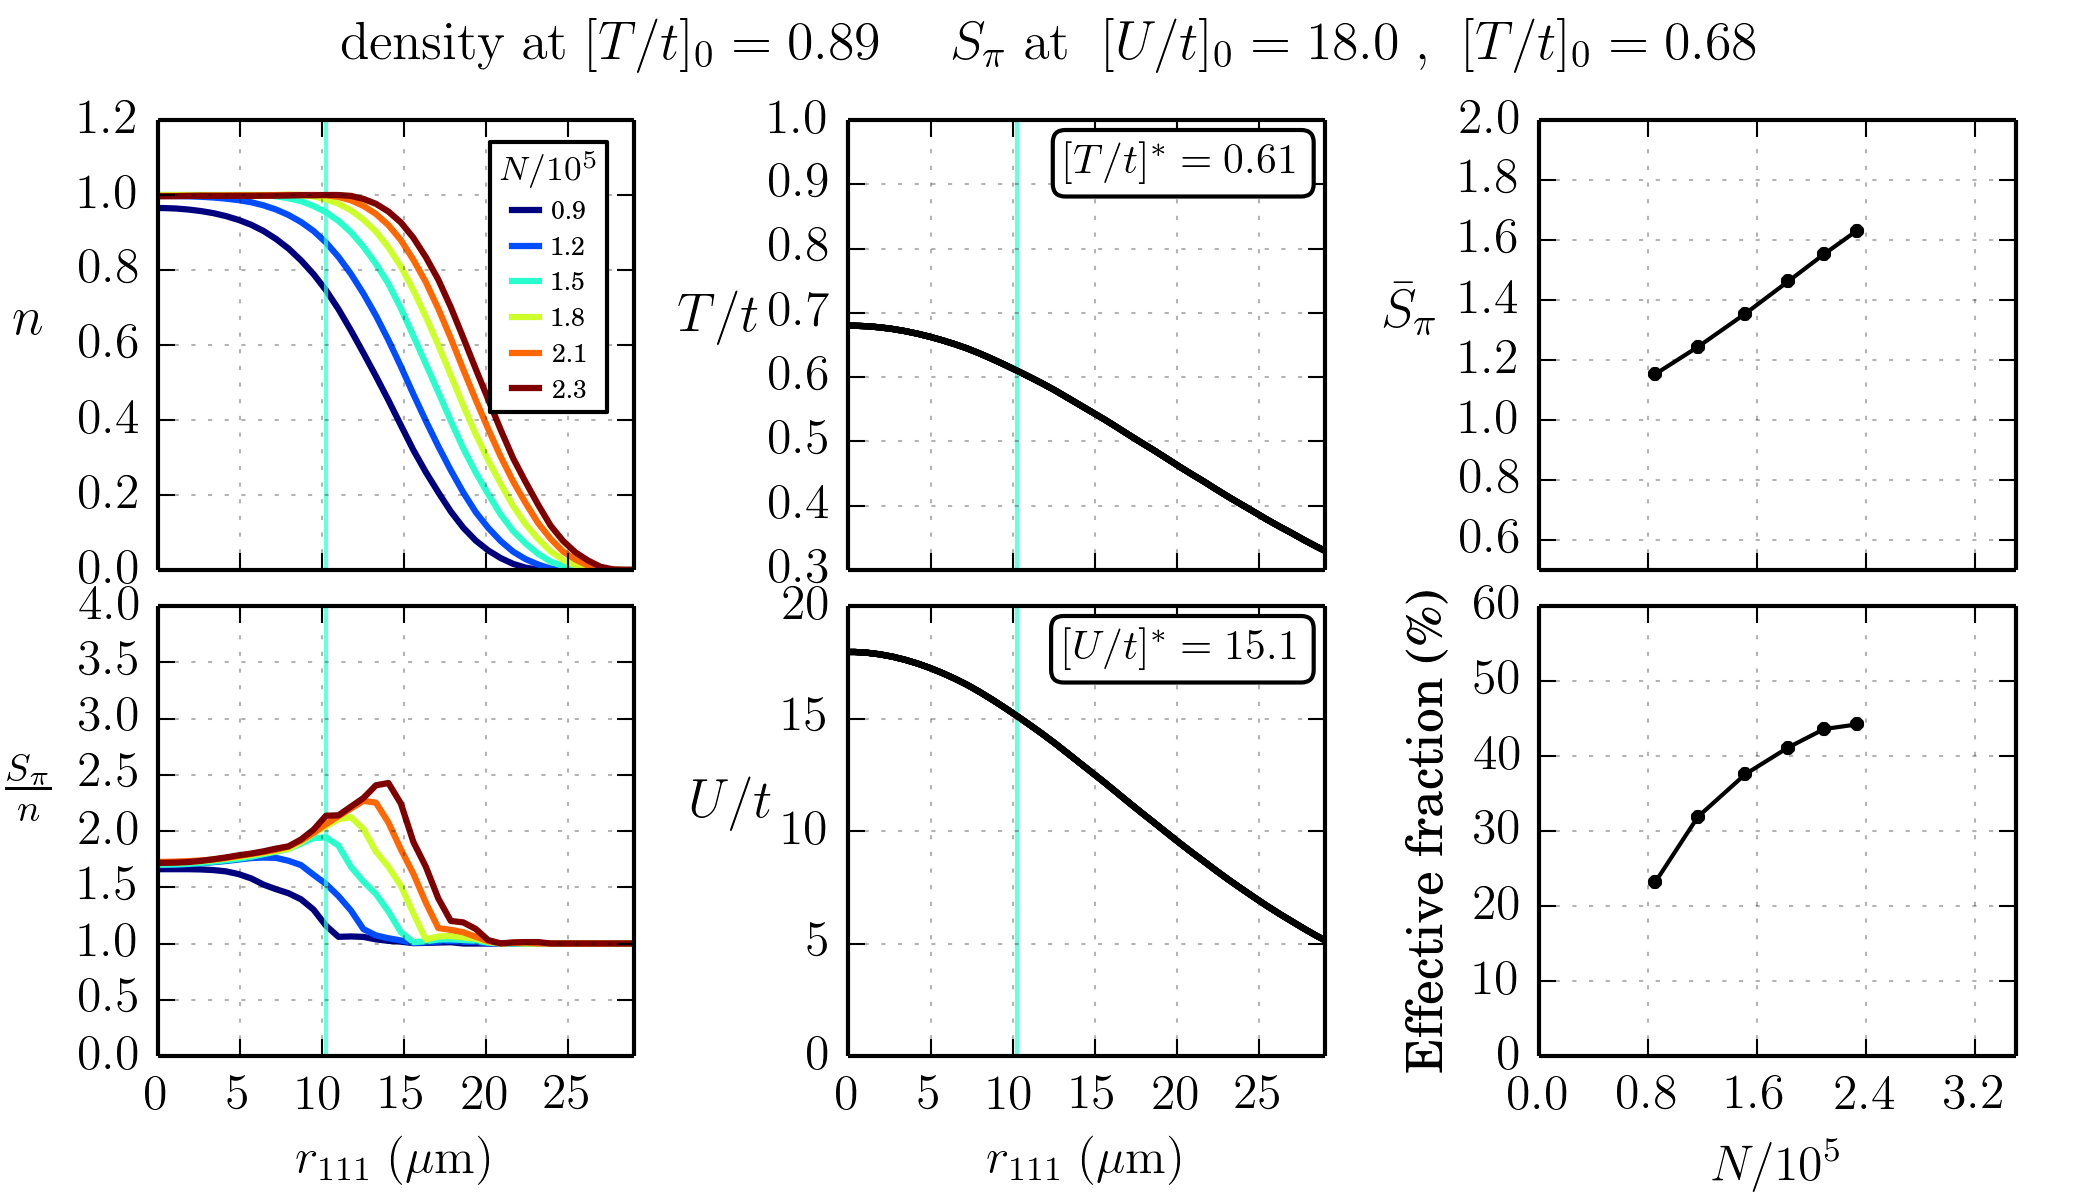
\includegraphics[width=\textwidth]{figures/470a0_cold.png}
\caption{Scattering length 470\,$a_{0}$ ($[U/t]_{0}=18.0$).   } 
\label{fig:470a0_varyN}
\end{figure}

The results for the lowest accessible values of $[T/t]_{0}$ are shown in
Figs.~\ref{fig:200a0_varyN}-\ref{fig:470a0_varyN}.   Even though there is data
available down to $T/t=0.36$ the lowest accesible $[T/t]_{0}$ is only 0.68
because as one moves radially outwards the local $T/t$ decreases.  We are
limited by the local value of $T/t$ at the edge of the cloud.   

Notice that in Figs.~\ref{fig:200a0_varyN}-\ref{fig:470a0_varyN} we indicate
values for $[T/t]^{*}$ and $[U/t]^{*}$, which are the local values of $T/t$ and
$U/t$ where $S_{\pi}/n$ is maximized.     

The main features that stand out from
Figs.~\ref{fig:200a0_varyN}-\ref{fig:470a0_varyN} are 
\begin{enumerate}

  \item Looking at weak interactions ($[U/t]_{0}=7.6$) we see that the peak in
$\bar{S}_{\pi}$  as a function of $N$ is much broader than what we have
observed in the experiment. 
 
  \item Looking at strong interactions ($[U/t]_{0}\geq 14.5$) we see that
$\bar{S}_{\pi}$ continues to increase with atom number.  For larger atom
numbers the contribution to the structure factor is coming from the outermost
shell of the cloud.   We are afraid that our spherical symmetry assumption may
not apply as far out from the center and that $\bar{S}_{\pi}$ should ultimately
decay with increasing atom number, as we observe in the experimental data.
\end{enumerate}

\subsection{ $\bar{S}_{\pi}$ vs. $N$ for various $T$'s} 

Finally we repeat calculations like those shown in
Figs.~\ref{fig:200a0_varyN}-\ref{fig:470a0_varyN} for several temperatures and
show the results for $\bar{S}_{\pi}$  in Fig.~\ref{fig:bulkSPI}.  Some comments
are included in the figure caption.  
\begin{figure}
    \centering
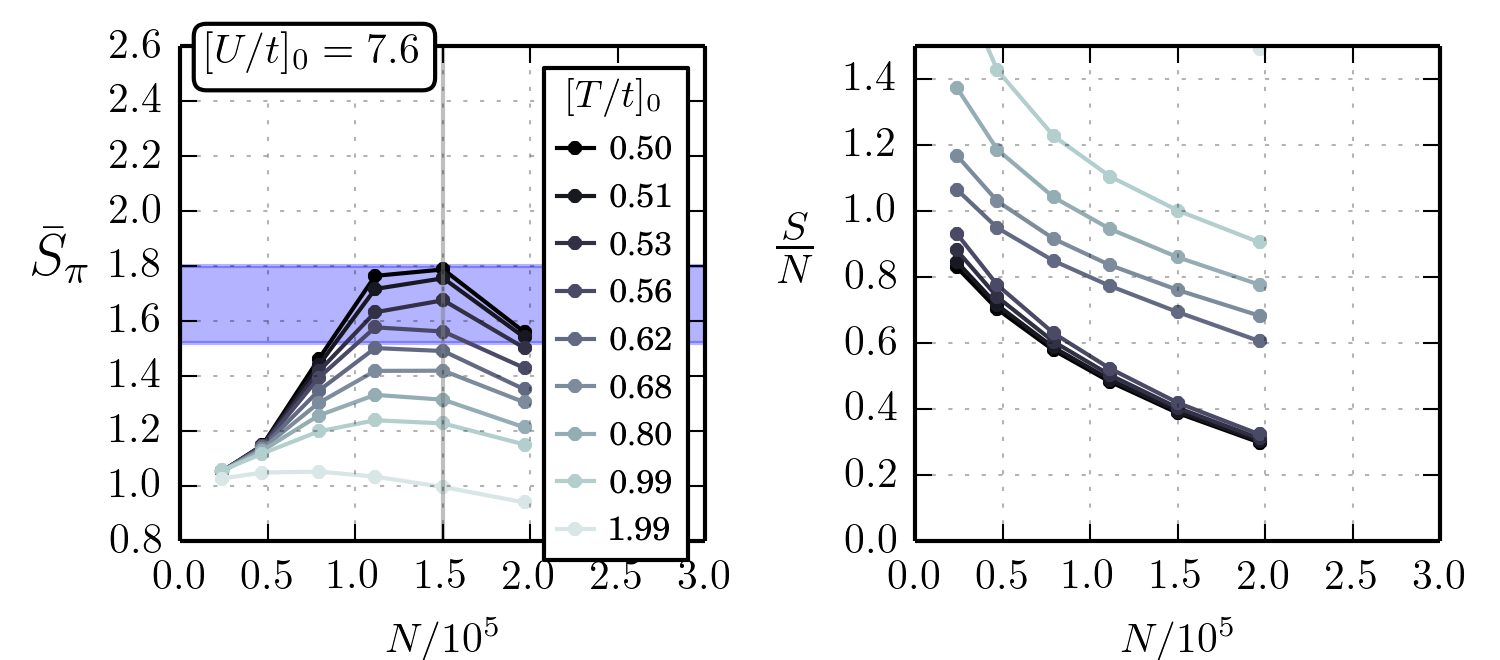
\includegraphics[width=0.48\textwidth]{../dataplots/SPI/200/spis.png}
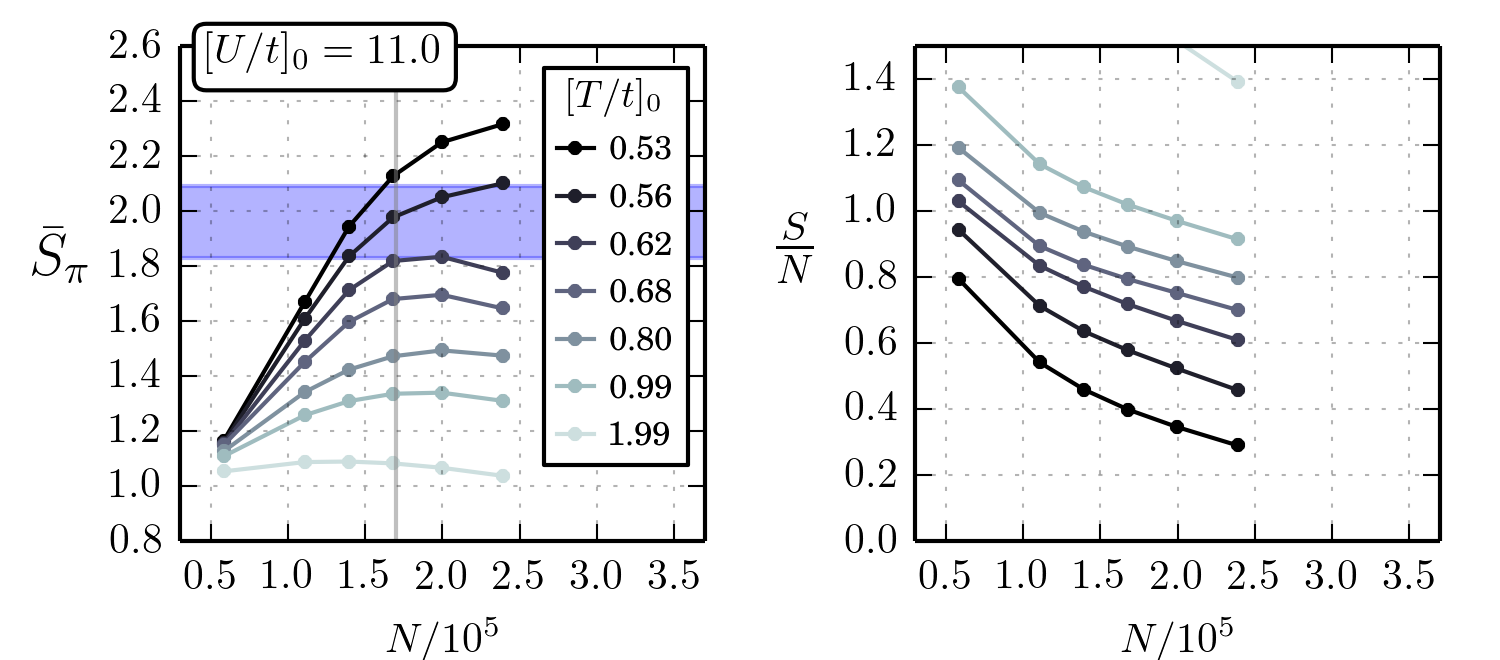
\includegraphics[width=0.48\textwidth]{../dataplots/SPI/290/spis.png}

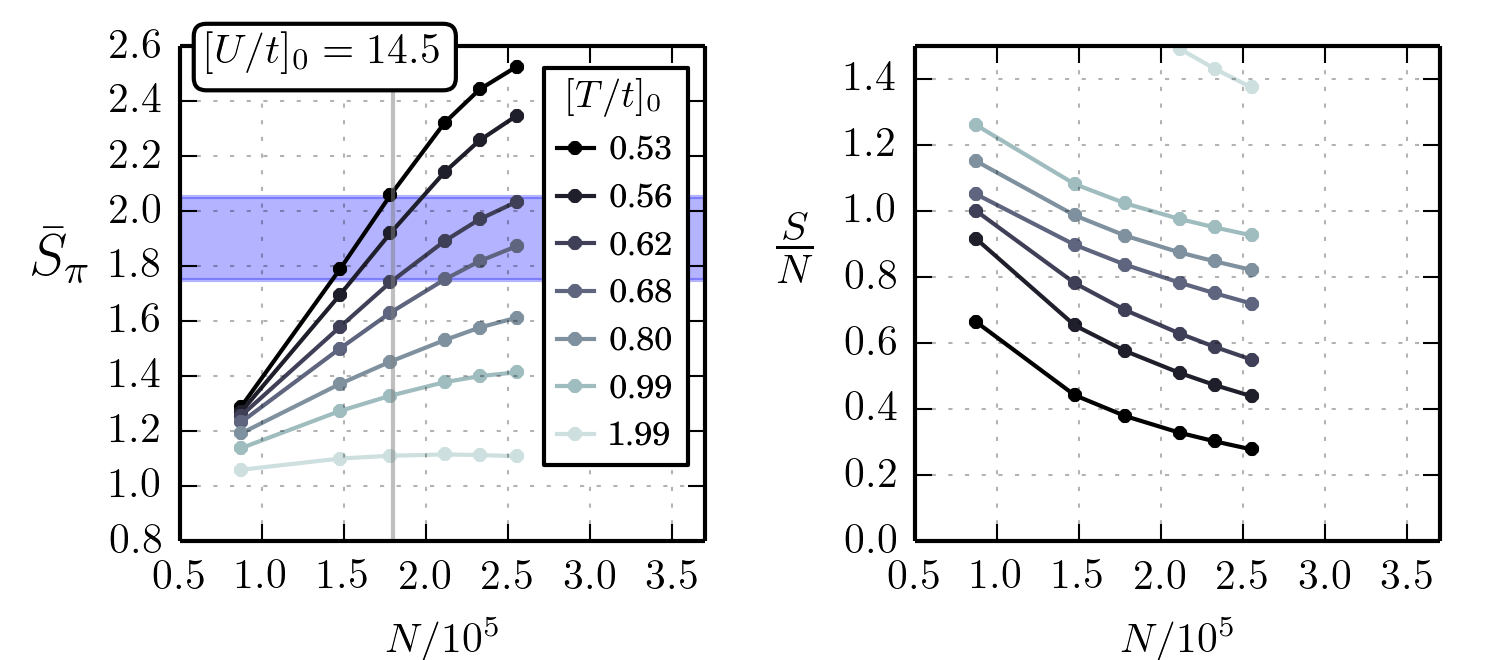
\includegraphics[width=0.48\textwidth]{../dataplots/SPI/380/spis.png}
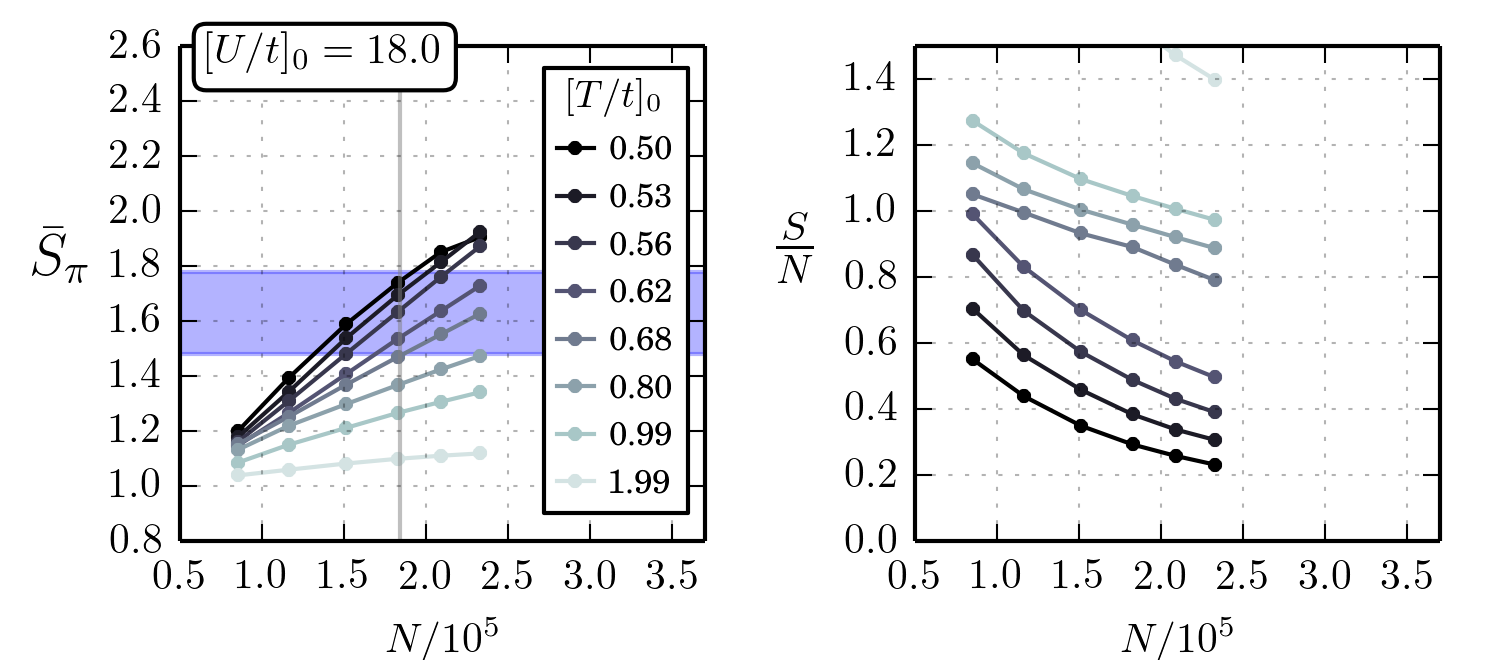
\includegraphics[width=0.48\textwidth]{../dataplots/SPI/470/spis.png} \caption{
Final comparison of experimental data with LDA.  The shaded blue area indicates
the experimental range for $\bar{S}_{\pi}$.  The vertical gray line indicates
the atom number at which the Bragg signal peaks up in the experiment.   For
larger atom numbers the spherical symmetry assumed in the LDA comes into
question.  We see that the lowest temperature accessible at the moment,
$[T/t]_{0}=0.68$, is not cold enough to reproduce the $\bar{S}_{\pi}$ observed
in the experiment for $[U/t]_{0}\leq 14.4$.  In the case of $[U/t]_{0}=17.9$ at
the value of $N$ relevant for the experiment (vertical gray line) the LDA at
$[T/t]_{0}=0.68$ just touches the experimental error bar.    } 
\label{fig:bulkSPI}
\end{figure}



 
 

 
\bibliographystyle{osa} \bibliography{latt_evap}

\end{document}




